% Template for ICIP-2015 paper; to be used with:
%          spconf.sty  - ICASSP/ICIP LaTeX style file, and
%          IEEEbib.bst - IEEE bibliography style file.
% --------------------------------------------------------------------------
\documentclass{article}
\usepackage{spconf,amsmath,graphicx}
\usepackage[utf8]{inputenc} % Suporte para acentuação sem necessidade dos comandos especiais.
\usepackage{amsmath,epsfig}
\usepackage[portuguese,algoruled,longend]{algorithm2e}
\usepackage{multirow}
\usepackage{MnSymbol}
\usepackage{wasysym}
\usepackage[table,xcdraw]{xcolor}
\usepackage[brazilian]{babel}
\usepackage{url}
\usepackage{float}
\usepackage{enumerate}
\usepackage{multicol}
\usepackage[numbered,framed]{matlab-prettifier}
\usepackage{soul,framed} %,caption
\usepackage{steinmetz}
\usepackage{subfigure}
\usepackage{lipsum}% for dummy text
\colorlet{shadecolor}{yellow}

% Template includegraphics
% \begin{figure}[H]
% 	\begin{center}
% 		\label{fig:11}
% 		\includegraphics[width=2.5in]{Figures/S02_Grafico_Ajustado.png}
% 		\caption{Gráficos da Situação 03 Ajustados}
% 	\end{center}
% \end{figure}

% Example definitions.
% -------------------
\def\x{{\mathbf x}}
\def\L{{\cal L}}

% Title.
% ------
\title{Prova 1 - Processamento de Sinais Biológicos}
%
% Single address.
% ---------------
\name{Davi de Alencar Mendes (\url{dmendes@aluno.unb.br}) - 16/0026415}
\address{Engenharia Eletrônica, UnB-FGA, Brasília, Brasil}

\begin{document}
\onecolumn
\maketitle

% \section{Introdução}\label{sec:intro}
% \lipsum[3]
% \section{Resultados}\label{sec:resultados}
% \begin{multicols}{2}
% \lipsum[2]
% \end{multicols}
% --------------------------------------------------------------------------
\section*{Questão 1 - \textit{QMF - Quadrature Mirror Filter Banks}}
\subsection*{A - Objetivo da filtragem QMF}
Inicialmente, a filtragem de decomposição tem como objetivo separa as componentes em frequência, discriminando entre aproximação (passa-baixas) e detalhes (passa-altas). Essa filtragem deve ser realizada de tal maneira que não haja perda de informação. Em termos da síntese, a filtragem tem o papel crucial em anular o termos de \textit{alias}, tornando a transformada linear e invariante no tempo (LTI).

\subsection*{B - Critérios de Reconstrução Perfeita}

Inicialmente tomamos como exemplo o QMF disposto a seguir (figura ~\ref{fig:qmf}).
\begin{figure}[H]
	\begin{center}
		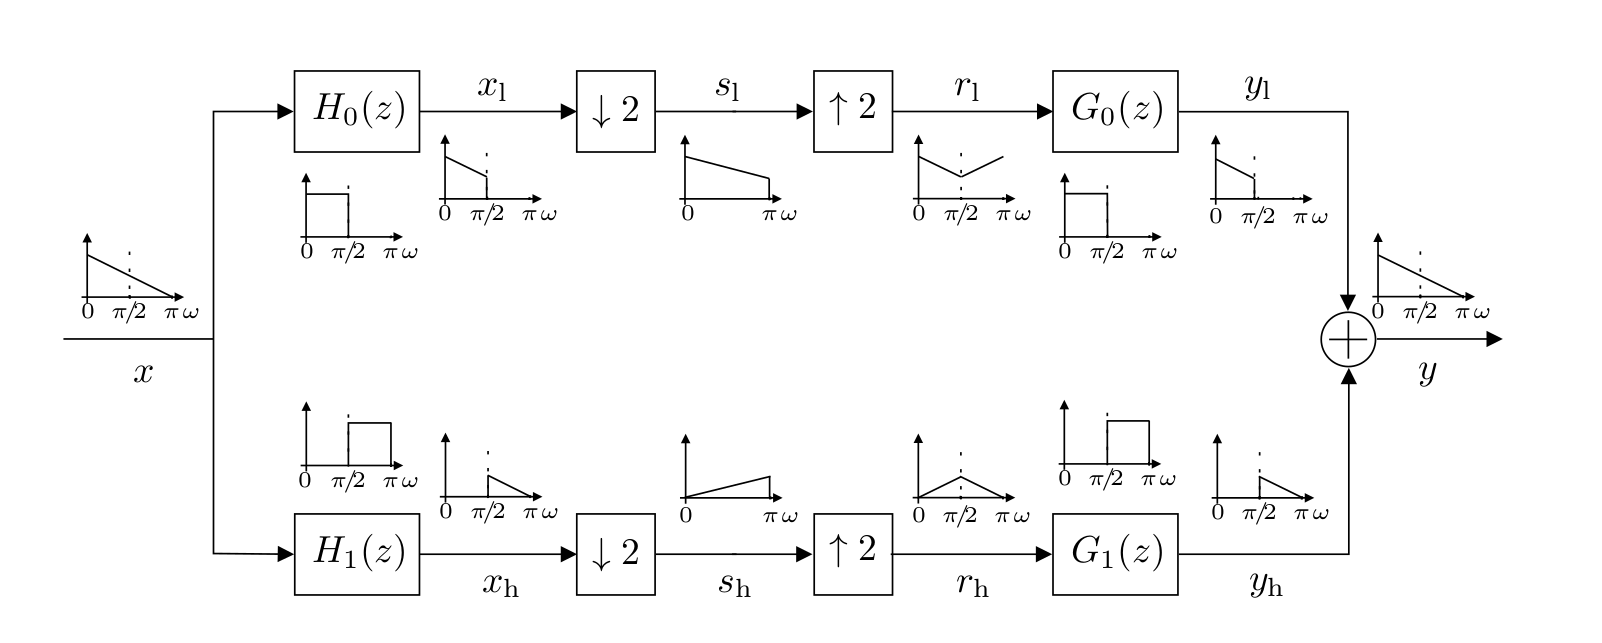
\includegraphics[scale=0.25]{Figures/qmf.png}
		\caption{QMF de 1 nível.}
		\label{fig:qmf}
	\end{center}
\end{figure}
Usando as identidades nobres dos blocos sub-amostradores e sobre-amostradores é possível obter as equações no domínio z para os pontos do QMF.
\begin{equation}
\begin{split}
x_1 = H_0(z)X(z) \\
s_1 = \frac{1}{2}[x_1(z^{1/2}) + x_1(-z^{1/2})] \\
s_1 = \frac{1}{2}[H_0(z^{1/2})X(z^{1/2}) + H_0(-z^{1/2})X(-z^{1/2})] \\
r_1 = s_1(z^2) \\
r_1 = \frac{1}{2}[H_0(z)X(z) + H_0(-z)X(-z)] \\
y_1 = \frac{1}{2} [G_0(z)H_0(z)X(z) + G_0(z)H_0(-z)X(-z)]
\end{split}
\end{equation}

De maneira análoga:
\begin{equation}
y_h = \frac{1}{2} [G_1(z)H_1(z)X(z) + G_1(z)H_1(-z)X(-z)]
\end{equation}

Dividindo as equações em termos de elementos variantes no tempo e invariantes e aplicando as condições de reconstrução perfeita obtemos:
\begin{equation}
\begin{split}
G_0(z)H_0(z) + G_1(z)H_1(z) = 2 \cdot A \cdot z^{-d} \\
G_0(z)H_0(-z) + G_1(z)H_1(-z) = 0
\end{split}
\end{equation}

Sendo estas as condições de reconstrução perfeita para o QMF de 1 nível.

\subsection*{C - Inversão dos filtros de síntese e análise}
Para a reconstrução perfeita foram obtidas um sistema de 2 equações e 4 filtros a serem obtidos. O problema original já apresenta infinitas soluções e ao adicionar mais uma equação para a inversão dos filtros de síntese e decomposição não altera o conjunto solução do problema.

\subsection*{D - Classificação do conjuntos de filtros}
Iniciamos a análise computando os zeros para o filtro $H_a$ sendo eles $1.02 \phase \pm 2.74^{\circ}$, $0.944 \phase 0^{\circ}$ e $0.3253 \phase \pm 151.99^{\circ}$. Pelo posicionamento dos zeros é possível constatar que se trata do filtro passa-altas de decomposição.

A inspeção do filtro $H_b$ mostra que trata-se de uma versão de ordem reversa e cópia modulada (\textit{reversed order \& modulated copy}) de $H_a$, ou seja, $h_b(n) = (-1)^n h_a(6-n)$. Adicionalmente $G_a(z) = -H_a(-z)$ e $G_b(z) = H_b(-z)$. Finalmente, pode-se concluir que se trata de um conjunto de reconstrução perfeita já que as condições de inversão dos coeficientes para os filtros de síntese indicam que tratam de versões passa-baixa e passa-altas para os filtros de decomposição.

Logo, $H_a$ é o filtro passa-alta de decomposição e $G_b$ é o filtro passa-baixa de síntese. $H_b$ é o filtro passa-baixa de decomposição de $G_a$ é o filtros passa-altas de síntese. Apesar de não estar citado, é de conhecimento do autor que os respectivos filtros são da família Daubechies (db3).

\subsection*{E - Ortogonalidade do conjunto de filtros}
Para provar a ortogonalidade usamos $\langle g_i(n)g_j(n) \rangle = \delta(i-j)$ para $i,j =\{0,1\}$. Iterando para i e j devemos encontrar:

\begin{equation}
\begin{split}
\sum_{n}^{} g_0^2(n) = \sum_{n}^{} g_1^2(n) = 1 \\
\sum_{n}^{} g_0(n)g_1(n) = 0
\end{split}
\end{equation}

Aplicando para $g_0(n) = g_a(n)$ e $g_1(n) = g_b(n)$:

\begin{equation}
\begin{split}
\sum_{n}^{} g_0^2(n) = 0.3327^2 +    0.8069^2 +    0.4599^2   -0.1350^2   -0.0854^2 +    0.0352^2 = 1 \\
\sum_{n}^{} g_0(n)g_1(n) = 0.0117+    0.0689   -0.0621+    0.0621   -0.0689   -0.0117 = 0
\end{split}
\end{equation}

Provamos que o conjunto é ortogonal e ortonormal. Por ser ortonormal também é bi-ortogonal. O resultado é análogo para os filtros de síntese.

\newpage
\subsection*{F - Diagrama Decomposição QMF de 3 níveis}
Utilizando as identidades nobres é possível reduzir o QMF de 3 níveis para a representação mostrada na figura ~\ref{fig:Q1_dec}.

\begin{figure}[H]
	\begin{center}
		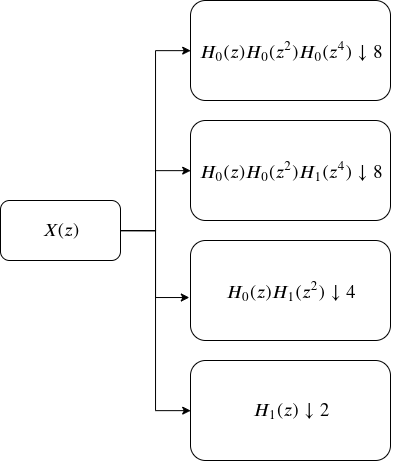
\includegraphics[scale=0.35]{Figures/dec_3.png}
		\caption{Decomposição QMF - 3 níveis}
		\label{fig:Q1_dec}
	\end{center}
\end{figure}

\subsection*{G - Diagrama Síntese QMF de 3 níveis}

\begin{figure}[H]
	\begin{center}
		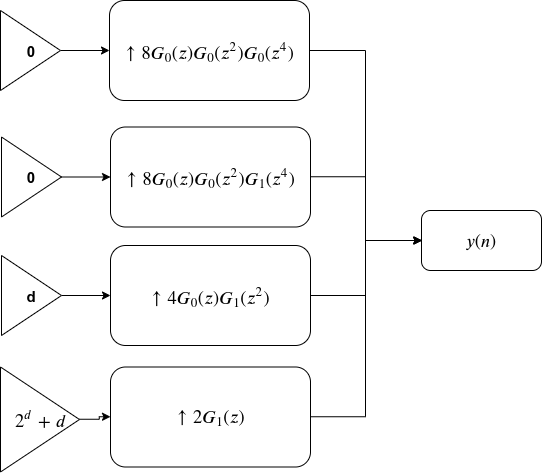
\includegraphics[scale=0.35]{Figures/rec_3.png}
		\caption{Síntese QMF - 3 níveis}
		\label{fig:Q1_rec}
	\end{center}
\end{figure}

\subsection*{H - Resposta em Frequência dos Filtros de Decomposição}

\begin{figure}[H]
	\begin{center}
		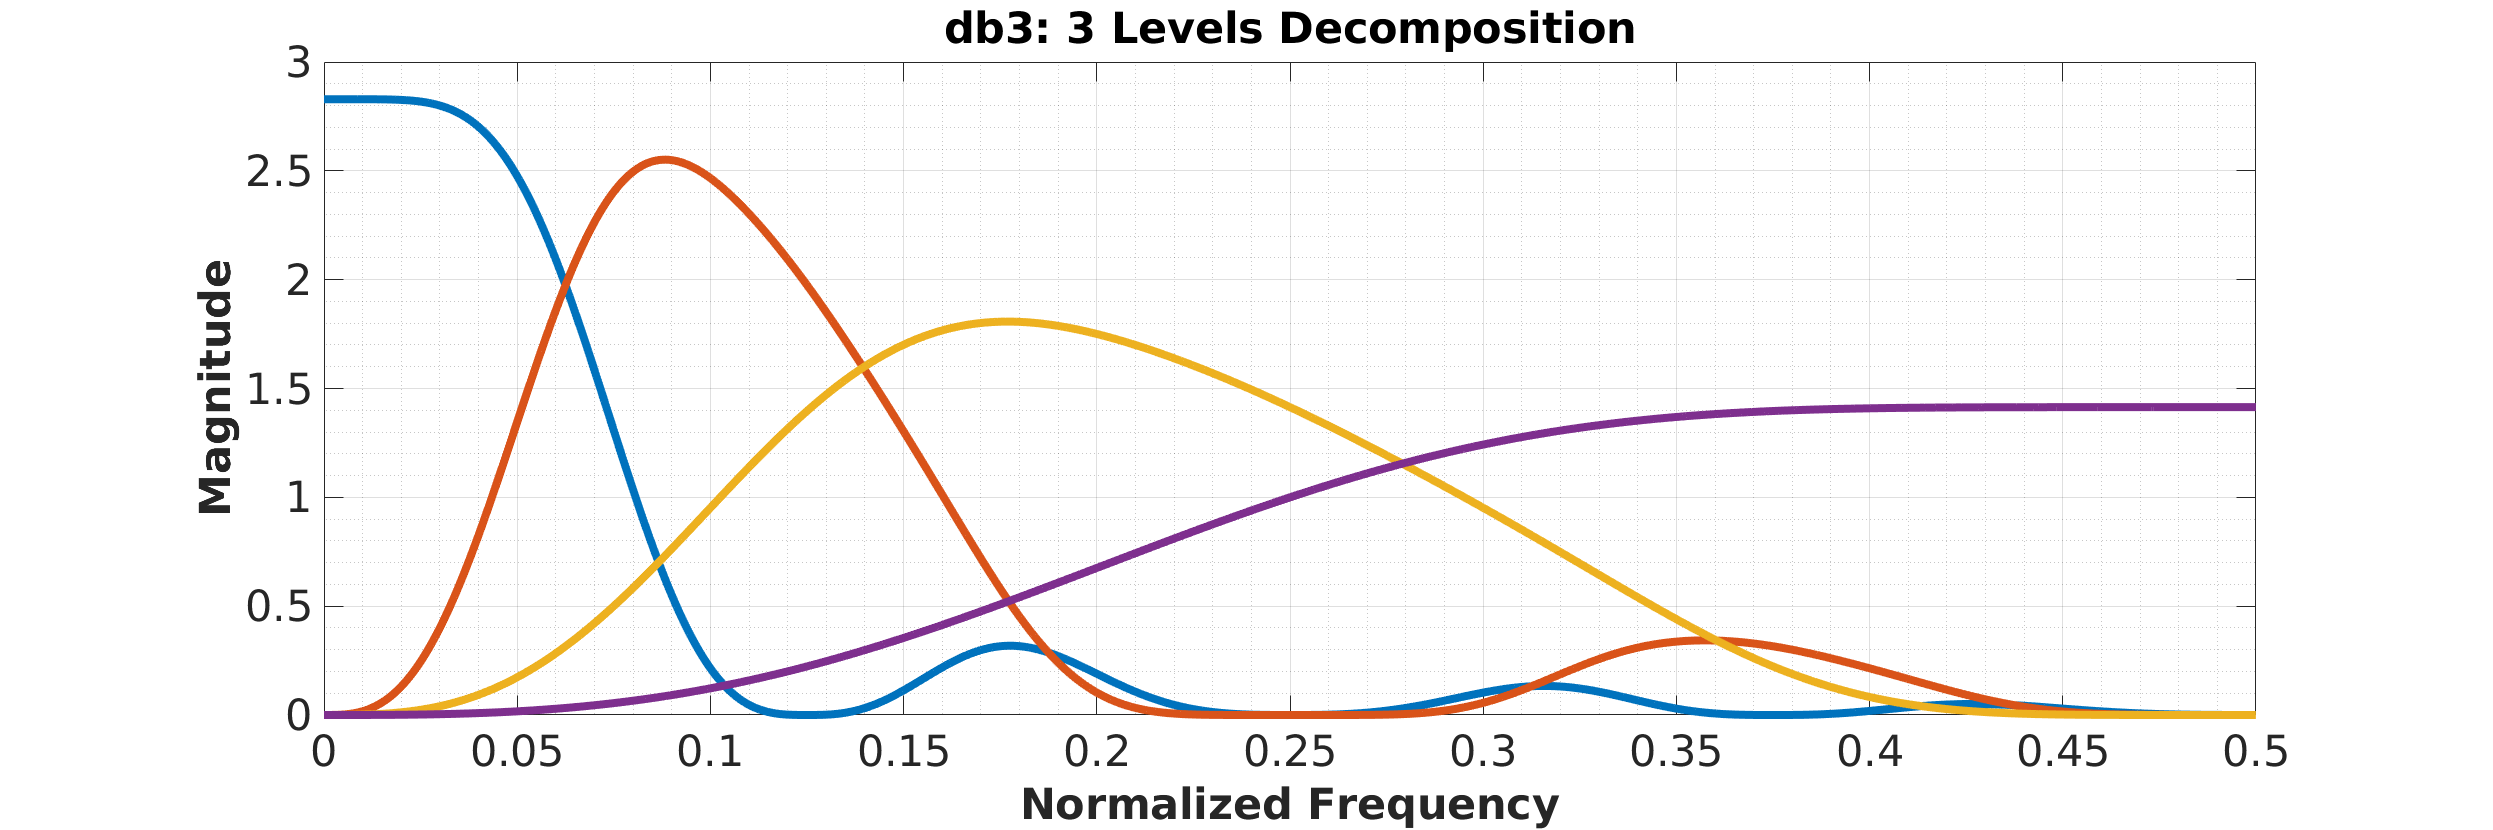
\includegraphics[scale=0.25]{../Q1_db3-3levels.png}
		\caption{Resposta em frequência - 3 níveis}
		\label{fig:Q1_db3_3}
	\end{center}
\end{figure}

\begin{figure}[H]
	\begin{center}
		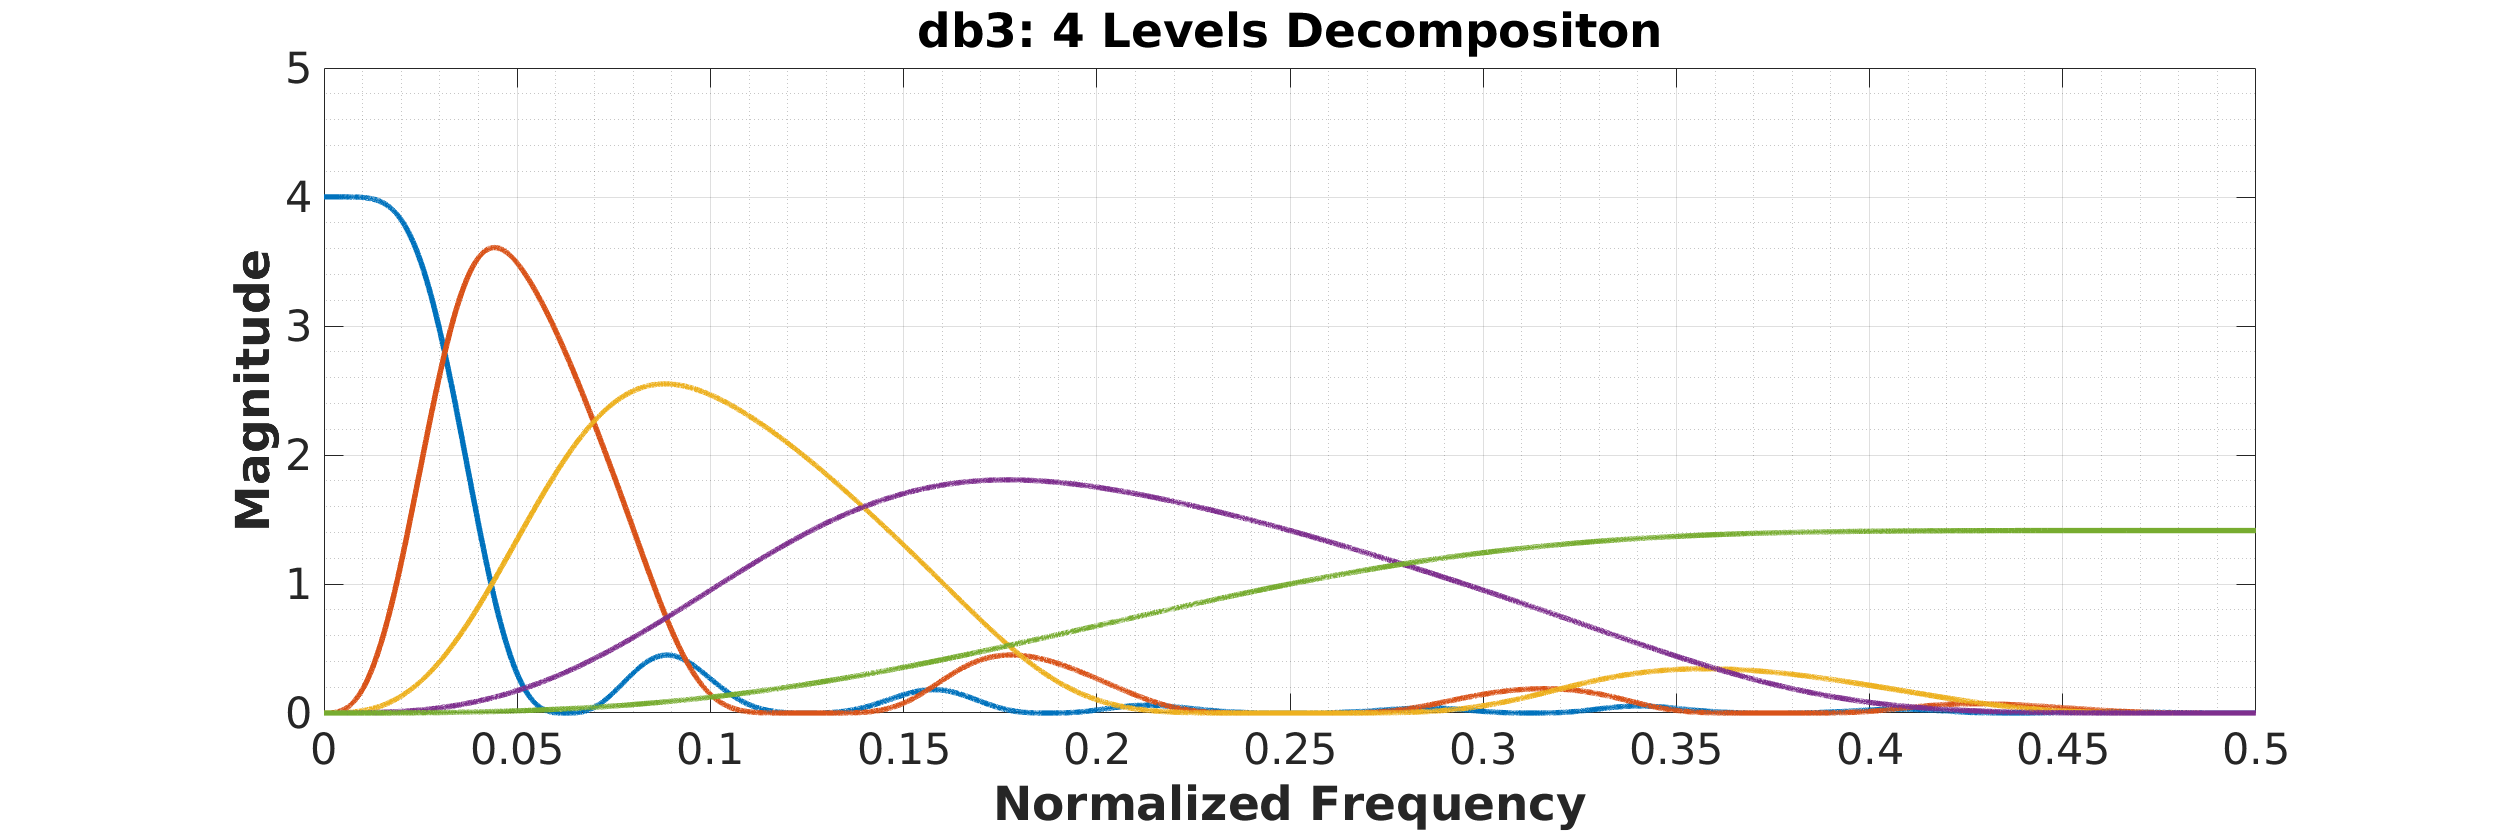
\includegraphics[scale=0.25]{../Q1_db3-4levels.png}
		\caption{Resposta em frequência - 4 níveis}
		\label{fig:Q1_db3_4}
	\end{center}
\end{figure}

\subsection*{I - Discussão acerca do item H}
Para as diferentes bandas de frequência mostradas é possível perceber que as bandas de baixa frequência são mais estreitas, algo que indica um comportamento de maior resolução no tempo na medida que bandas de maior frequência são mais espalhadas e superpostas mostrando que há maior resolução no tempo. A representação multinível é interessante por ressaltar tanto as características em frequência como temporais já que cada nível de decomposição gera uma representação diferente.

\subsection*{J - Escolha de conjunto de filtros}
É interessante lembrar que a adoção do conjunto de filtros é uma representação transformada na qual adotam-se bases para o sinal. Nesse sentido, há bases que são mais interessantes por ressaltar características particulares do sinal. Em especial para as wavelets, que codificam diferenças, é crucial ter conjuntos variados que sejam adaptáveis para diferentes cenários de aplicações.

\subsection*{K - Comparativo entre filtros}
A família de wavelets de Daubechies (db) possui propriedades de assimetria, ortogonalidade e biortogonalidade. A família de Coiflets apresenta quasi-simetria, ortogonalidade e biortogonalidade. A família de Symlets mantém as propriedades das Coiflets. A família Biortogonal é simétrica e biortogonal.

% --------------------------------------------------------------------------
\section*{Questão 2 - Análise de Sinais de ECG \& EMG}
\subsection*{A - Transformada de Fourier dos Sinais}
\begin{figure}[H]
	\begin{center}
		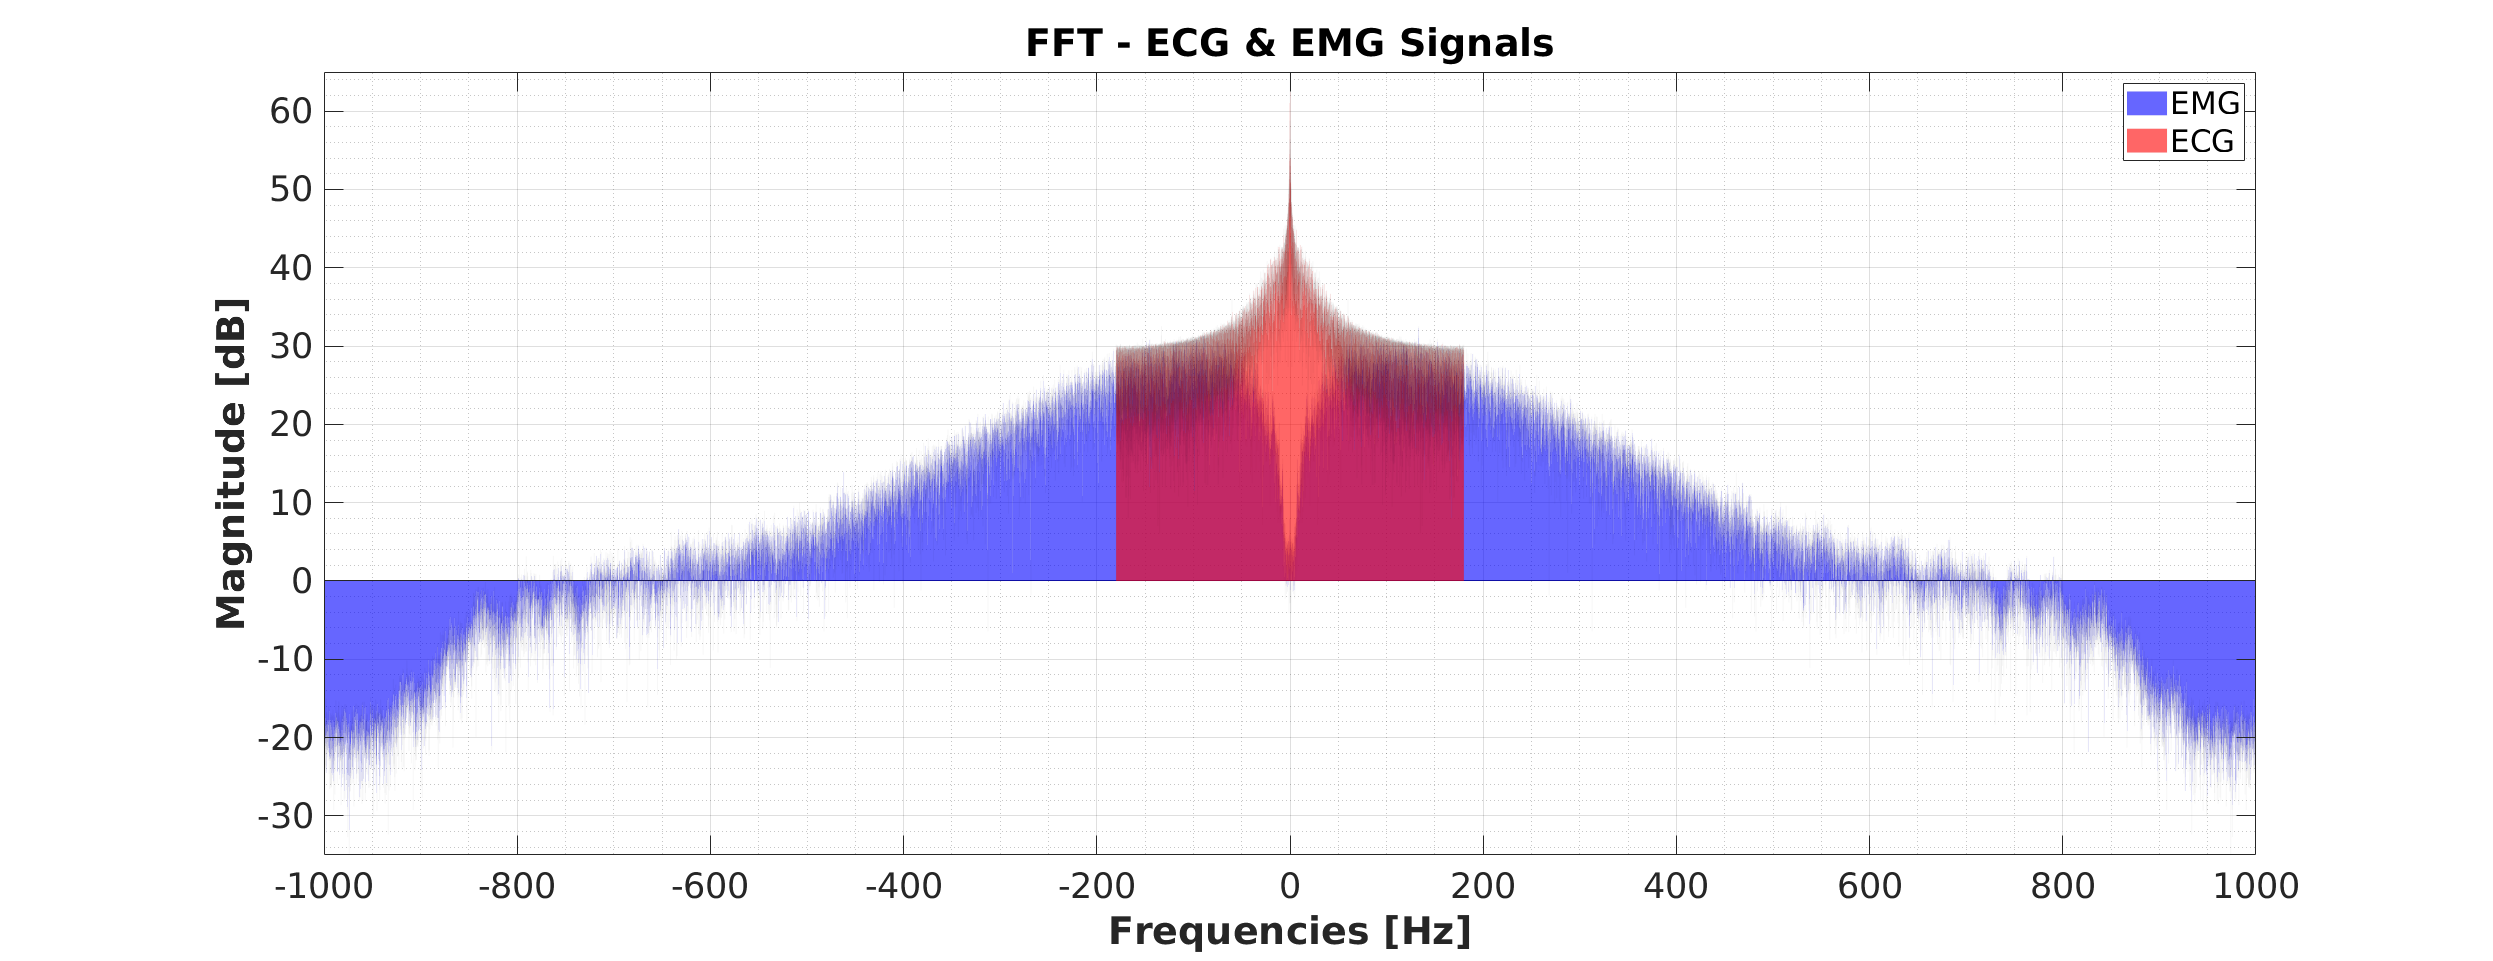
\includegraphics[scale=0.25]{../Q2_FFT_EMG-ECG.png}
		\caption{Transformada de Fourier para ECG \& EMG}
		\label{fig:Q2_FFT}
	\end{center}
\end{figure}

\begin{multicols}{2}
\subsection*{B - Largura de Banda: ECG vs EMG}
Tomando como ponto de partida a visualização gráfica de ~\ref{fig:Q2_FFT}, pode-se perceber que o sinal de ECG está contido majoritariamente entre 0-50 Hz. Já para o sinal de EMG percebe-se que sua largura de banda estende-se até 700 Hz com magnitude considerável. Claramente o sinal de ECG apresenta variações mais lentas no tempo na medida que o sinal de EMG apresenta variações mais aceleradas.
\subsection*{C - Percentual de Energia por Banda}
Foi computado um percentual de 88\% da energia total para a banda de 2-150 Hz no sinal de EMG. Ademais, o sinal de ECG apresenta 74\% da energia total para a banda de 2-40 Hz em sua versão com valor médio nulo. O procedimento de remoção do valor médio foi realizado já que os sinais de ECG e EMG apresentavam valores médios distintos, algo que poderia levar a uma análise errônea da energia total do sinal.
\subsection*{D - Discussão a respeito do item C}
Por apresentar variações mais rápidas no domínio do tempo é esperado que ocorra uma maior largura de banda do sinal de EMG considerado.
\subsection*{E - Formação de Ruído}
Durante a aquisição de sinais eletrofisiológicos é comum ocorrer contaminação com o sinal presente da rede elétrica (60Hz) já que, geralmente, o ambiente de coleta está sujeito a presença de outros equipamentos elétricos conectados em sua proximidade. Para o sinal considerado é possível notar que há um pico em 60 Hz com uma amplitude de +3 dB em relação ao nível da vizinhança.

A linha de base se dá em razão de sinais de baixa frequência proveniente do sistema respiratório (movimento muscular da respiração). O sistema de aquisição também pode gerar um offset de entrada na amostragem dos dados.
\end{multicols}

\subsection*{F - Filtragem com a DFT}
Para remover a linha de base foi escolhido filtrar entre 0-5 Hz e 58-62 Hz para remoção da interferência da rede elétrica. Considerando a versão não deslocada da FFT, podemos calcular o índice correspondente a uma frequência usando $index = round(f_c * N /fs )$ no qual $f_c$ denota a frequência desejada e N o comprimento correspondente da transformada do sinal. Para as frequências negativas utiliza-se $index = round((f_s - f_c) * N /fs )$ já que há a simetria na representação da magnitude. Para o sinal, foi calculada a FFT com 32768 pontos (próxima potência de 2 em relação ao comprimento do sinal de EMG) e foram eliminados os índices entre 1-456/32313-32768 para as frequências de 0-5 Hz e 5280-5644/27126-27409 para as frequências de 58-62 Hz.
\begin{figure}[H]
	\begin{center}
		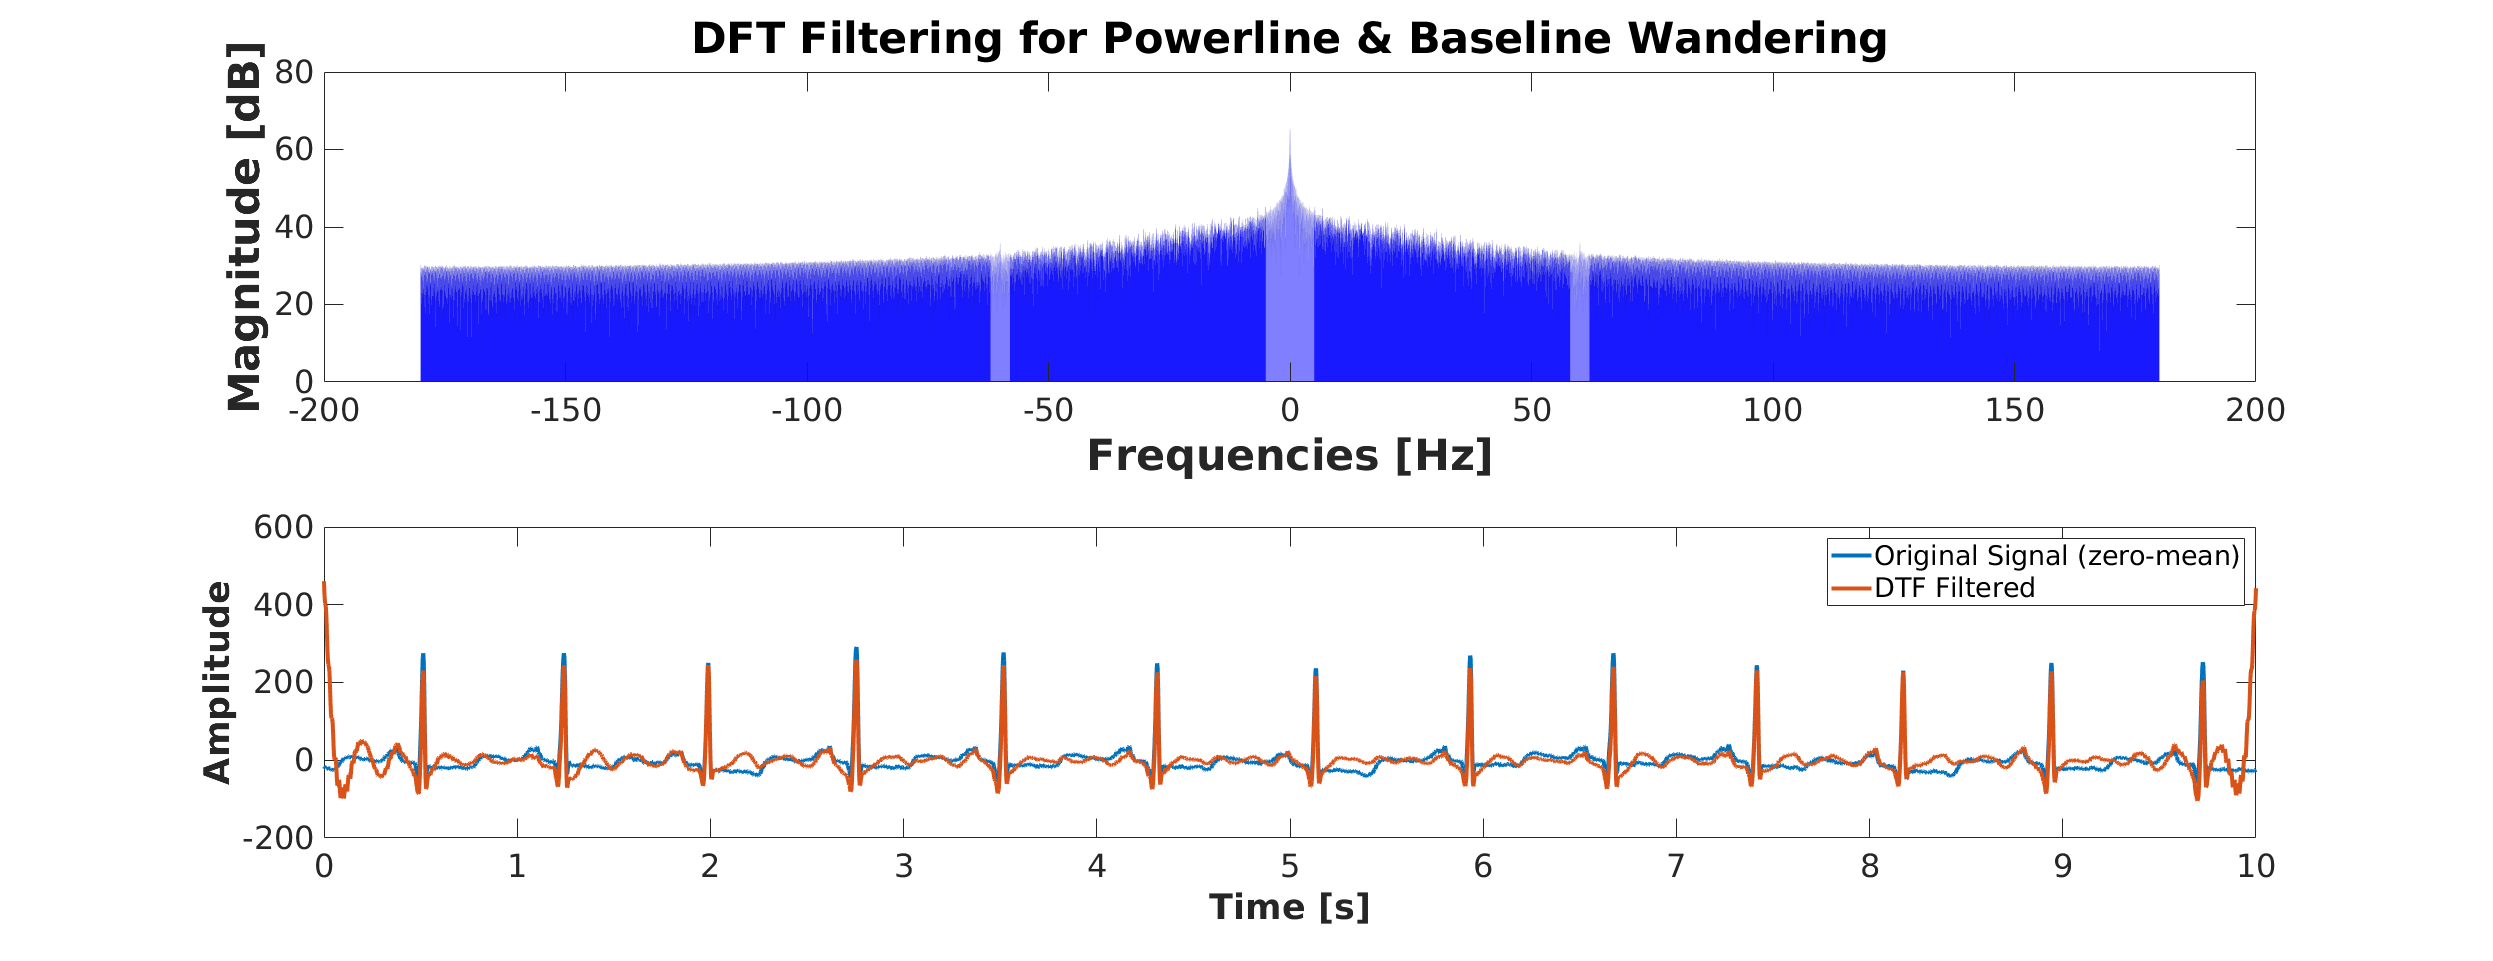
\includegraphics[scale=0.25]{../Q2_DFT-Filter-Time.png}
		\caption{DFT do Sinal e versão filtrada via DFT sobreposta a DFT original \& Sinais no domínio do tempo filtrados}
		\label{fig:Q2_DFT}
	\end{center}
\end{figure}

\subsection*{G - Filtragem FIR}
Após algumas iterações de análise visual dos sinais filtrados, foi considerado que filtrar com um filtro de ordem 150, sendo passa altas para 8 Hz e rejeita faixa entre 56 e 64 Hz. Os resultados da filtragem são expostos na figura ~\ref{fig:Q2_DFT}. A resposta em frequência pode ser vista na figura ~\ref{fig:Q2_FV}.

\begin{figure}[H]
	\begin{center}
		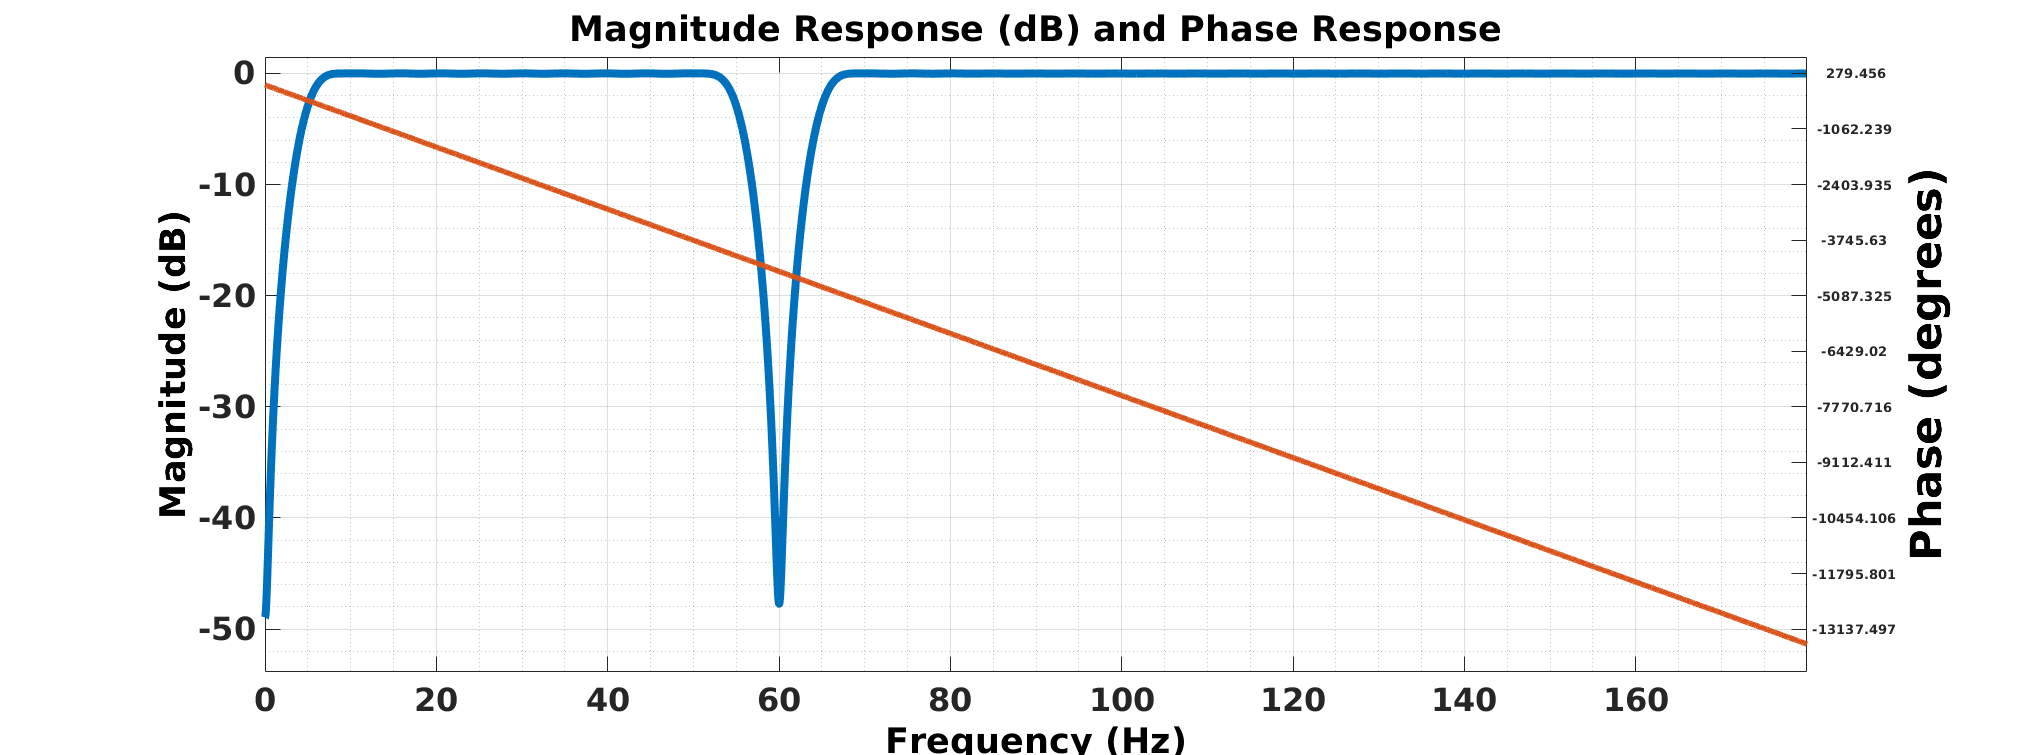
\includegraphics[scale=0.25]{../Q2_fvtool.png}
		\caption{Resposta em frequência e fase para o filtro FIR concebido}
		\label{fig:Q2_FV}
	\end{center}
\end{figure}

\begin{figure}[H]
	\begin{center}
		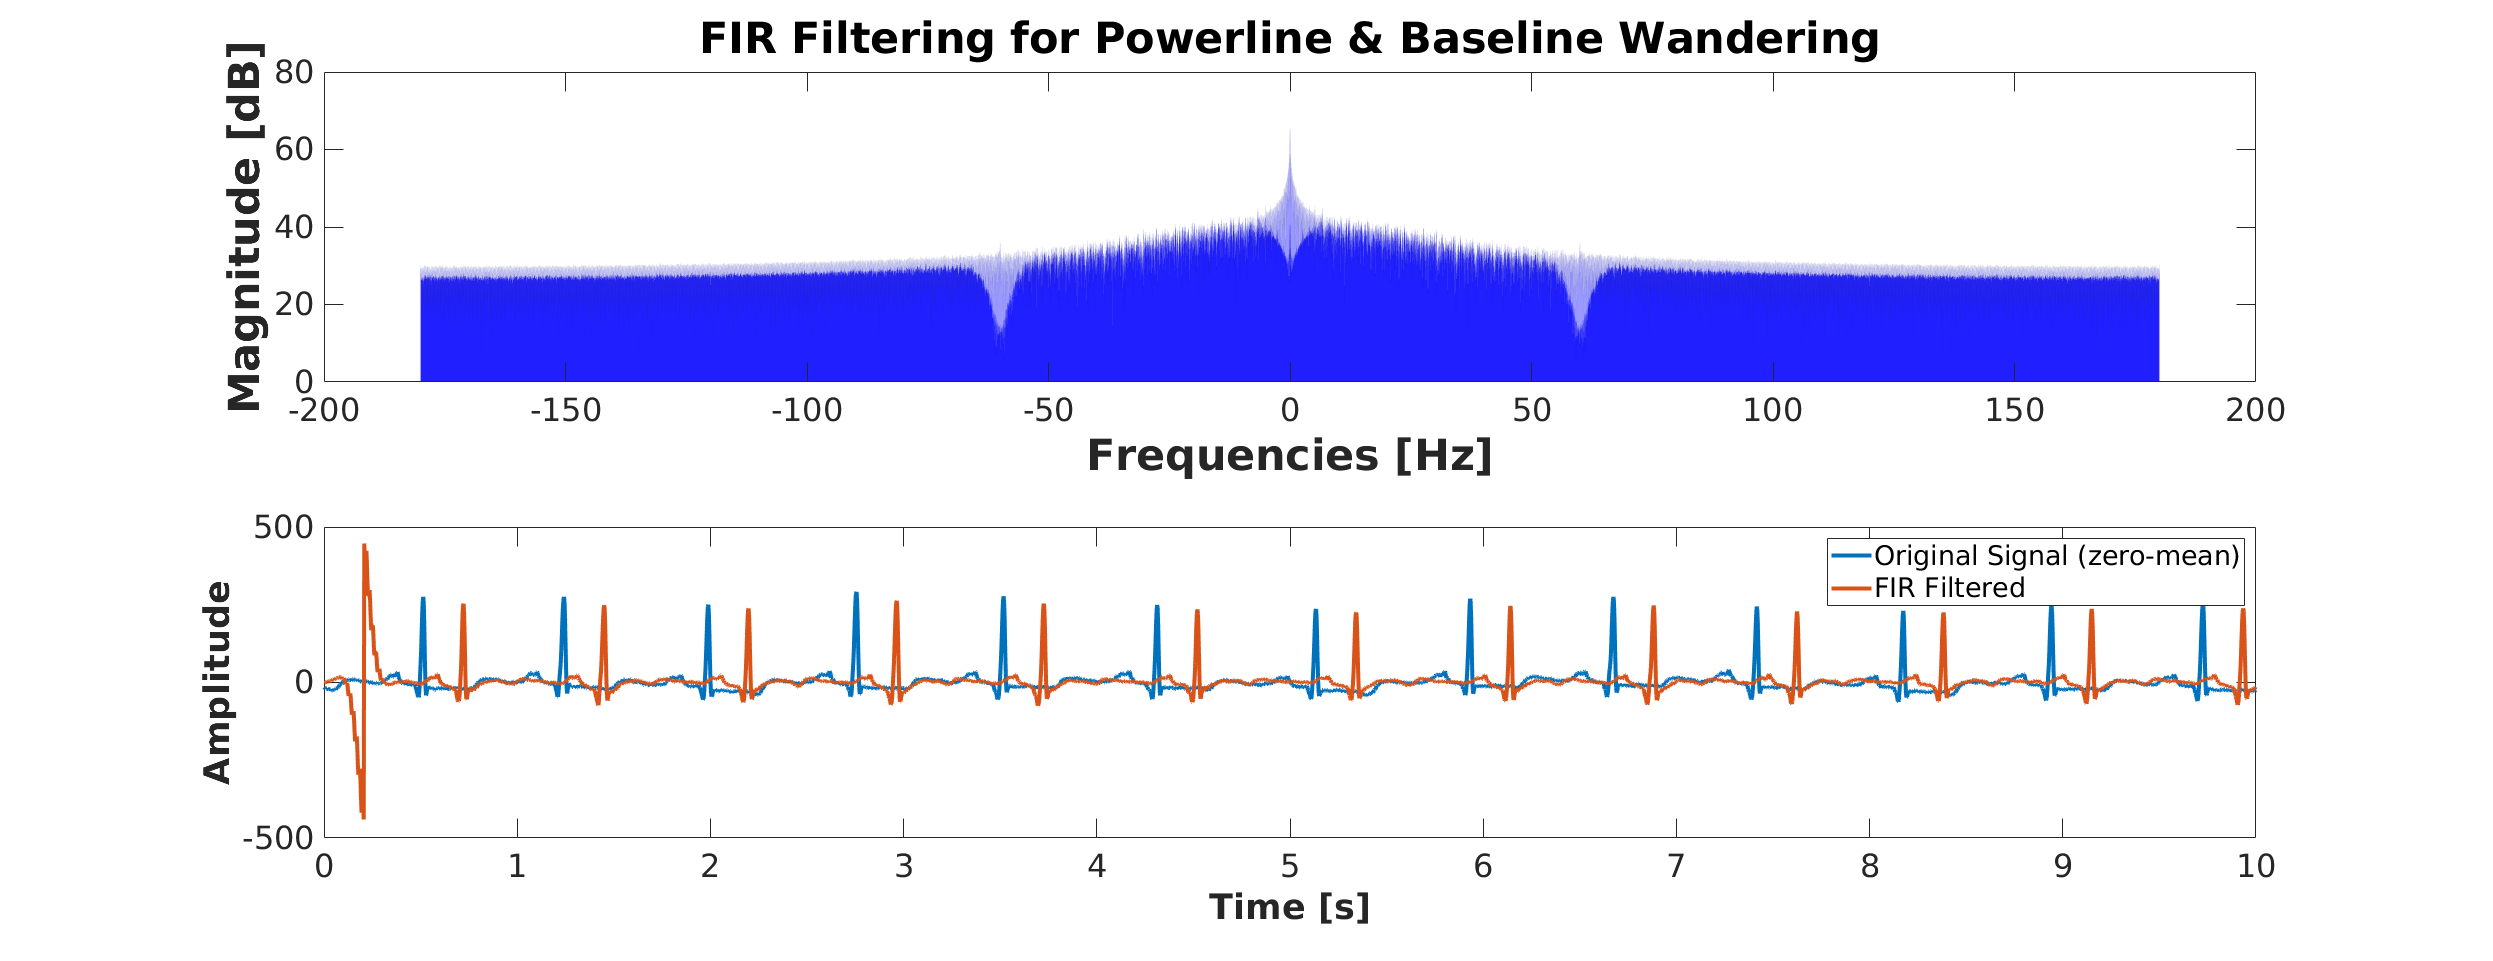
\includegraphics[scale=0.25]{../Q2_FIR-Filter-Time.png}
		\caption{DFT do Sinal e versão filtrada via FIR sobreposta a DFT original \& Sinais no domínio do tempo filtrados}
		\label{fig:Q2_FIR}
	\end{center}
\end{figure}
% --------------------------------------------------------------------------
\section*{Questão 3 - Transformada de Fourier \& Wavelets}
\subsection*{A - Transformada de Fourier do Sinal de EMG}

\begin{figure}[H]
	\begin{center}
		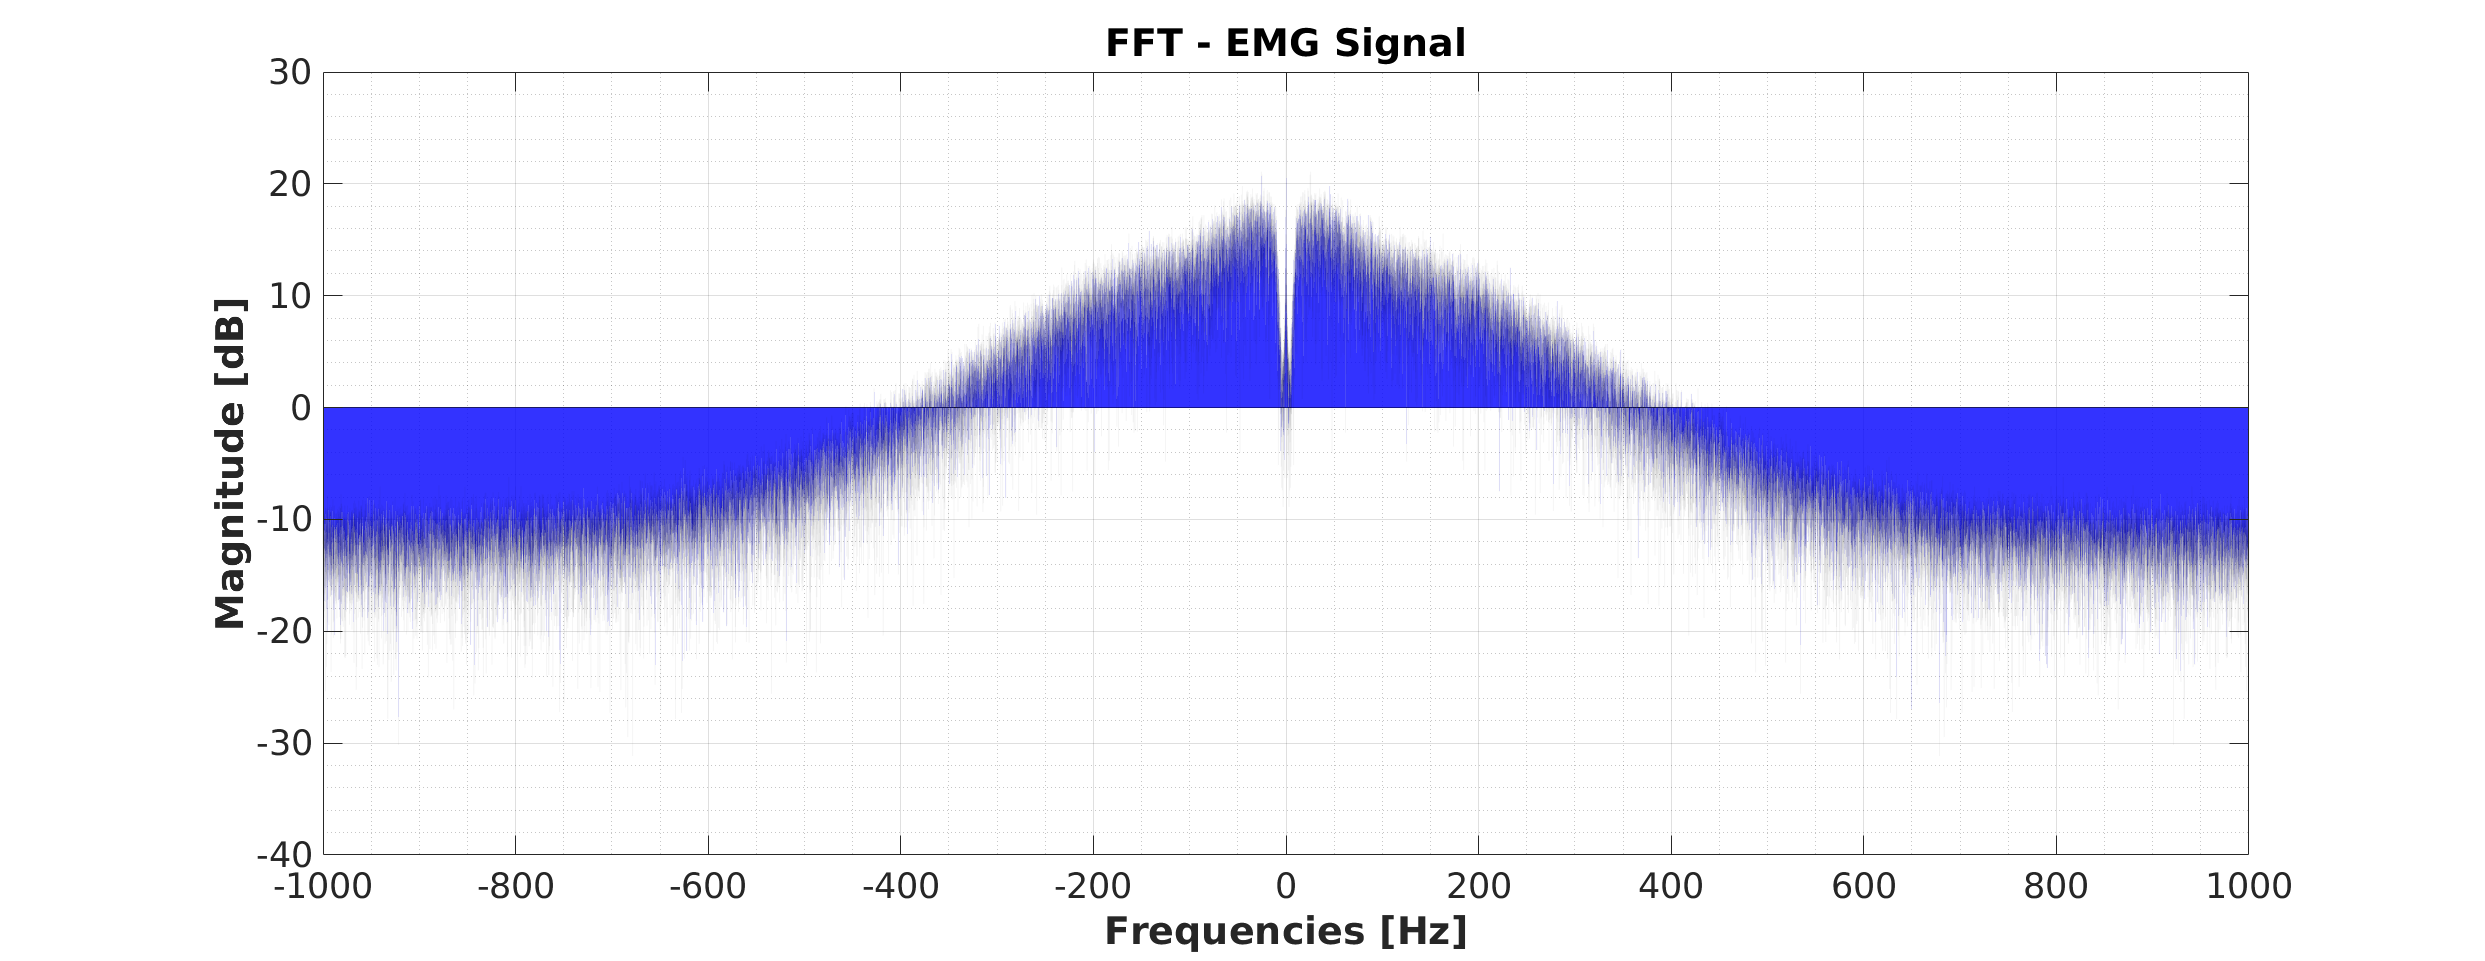
\includegraphics[scale=0.25]{../Q3_FFT.png}
		\caption{Magnitude da Transformada de Fourier do Sinal de EMG}
		\label{fig:Q3_FFT}
	\end{center}
\end{figure}

\subsection*{B - Adição de Eventos Senoidais de Alta Frequência}

Para adicionar os eventos senoidais de alta frequência foi desenvolvida uma função que recebe o sinal de entrada, taxa de amostragem, ponto inicial do evento e duração em segundos além das frequências para as harmônicas e o percentual de energia máximo relativo a energia do sinal durante a duração do evento. \textbf{É importante ressaltar que os eventos (200 senoides de frequências linearmente espaçadas) foram adicionados em intervalos de 1 segundos nos segundos: (1,2,3) do sinal de EMG.}

\lstinputlisting[style=Matlab-editor]{../aditiveHarmonicNoise.m}

\subsection*{C - Transformada de Fourier para EMG com Eventos}

\begin{figure}[H]
	\begin{center}
		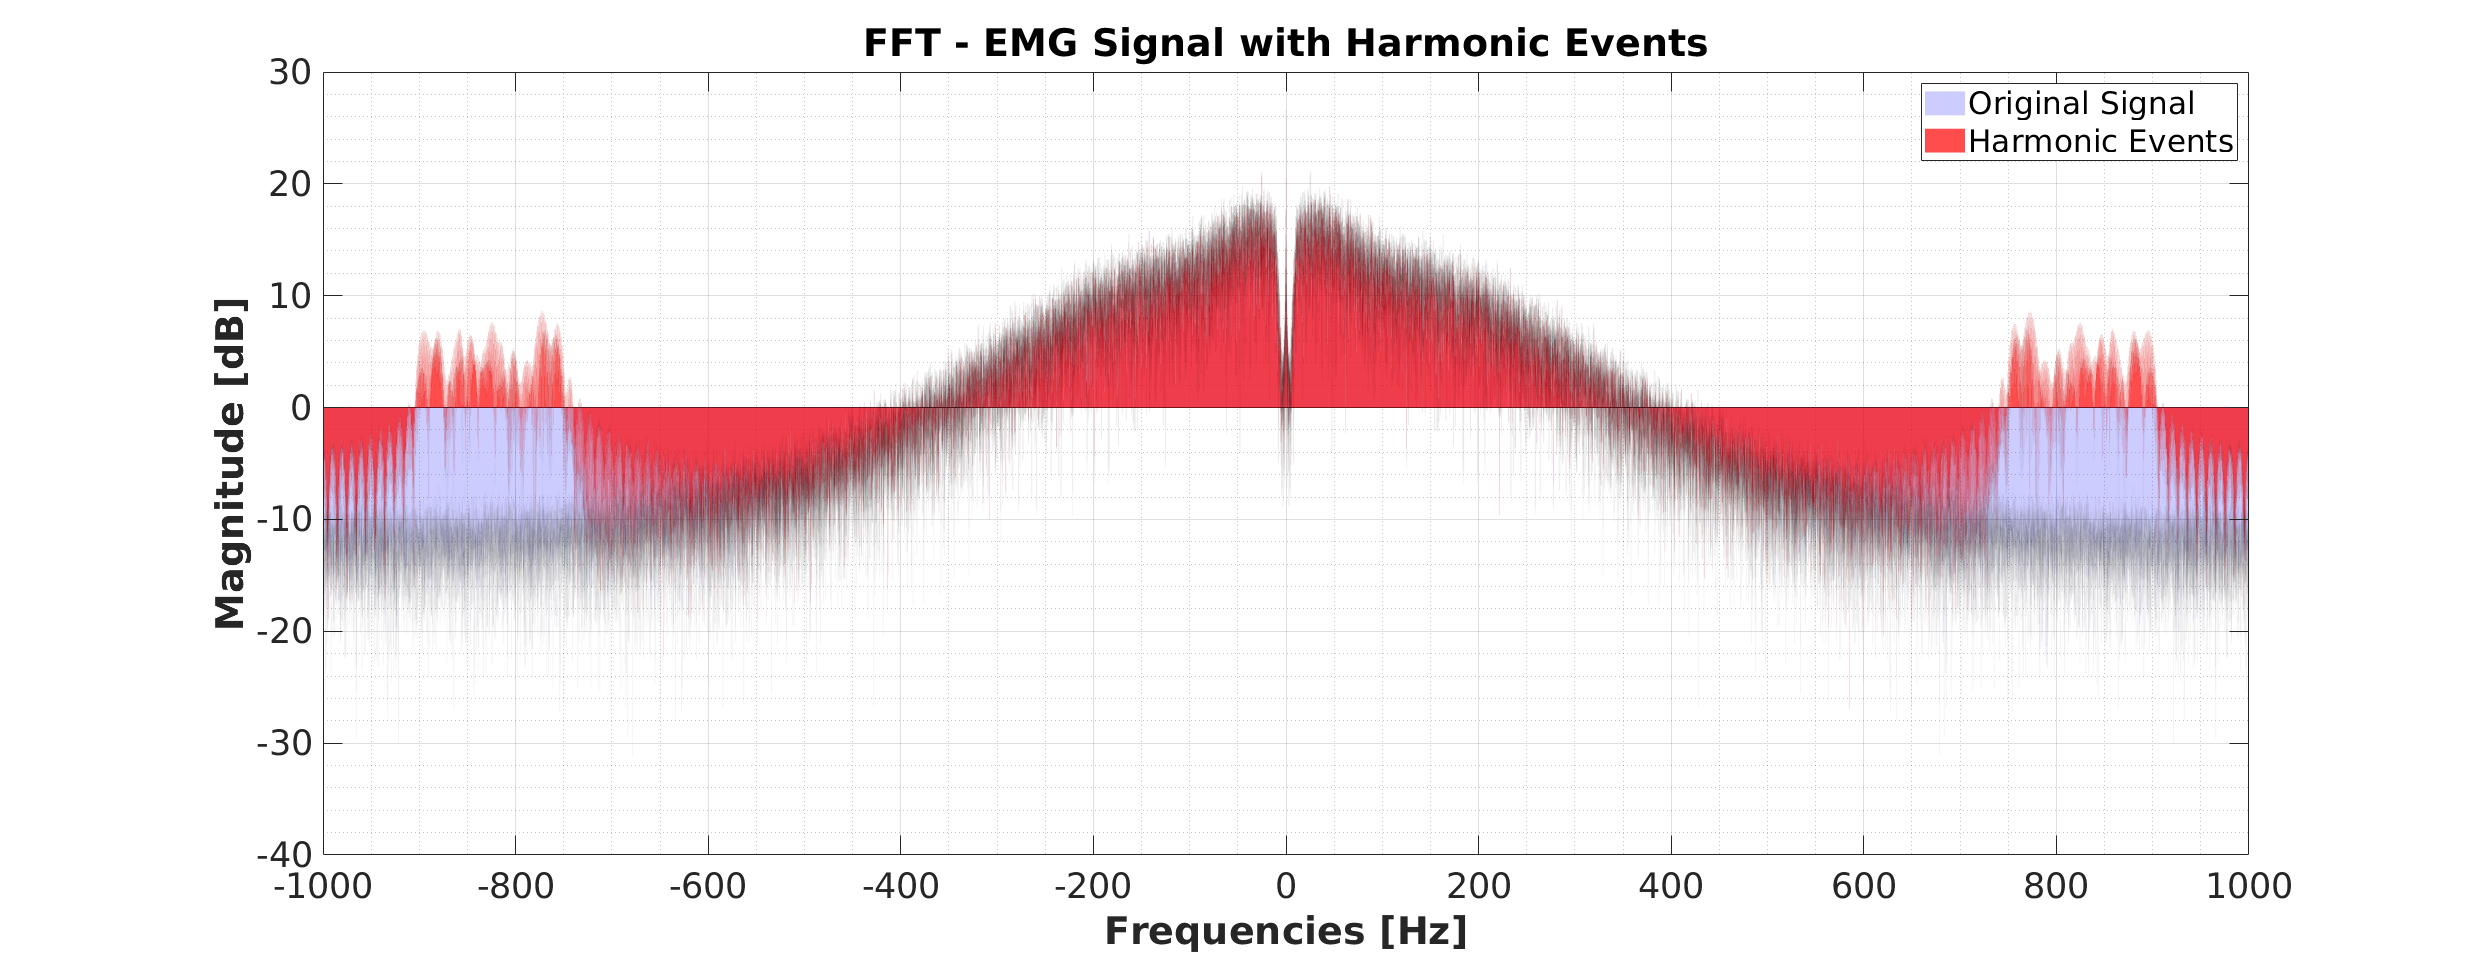
\includegraphics[scale=0.25]{../Q3_FFT-Events.png}
		\caption{Magnitude da Transformada de Fourier do Sinal de EMG \& Adição de Eventos Senoidais de Alta Frequência}
		\label{fig:Q3_FFT2}
	\end{center}
\end{figure}


Comparando a figura \ref{fig:Q3_FFT} com \ref{fig:Q3_FFT2} é possível notar que há conteúdos de alta frequência presentes no sinal mas é impossível distinguir o instante em que ocorrem os eventos no tempo. Embora a informação acerca dos instantes em que tais eventos ocorrem esteja embutida na fase da transformada este não é um dado de fácil interpretação.

\subsection*{D - Transformada Discreta de Wavelets: Daubechies 2 \& Discrete Meyer com 3 níveis}
Para observar os conteúdos de alta frequência do sinal deve-se observar o comportamento presente na menor escala para as figuras \ref{fig:Q3_DWT} e \ref{fig:Q3_DWT2}. Diferentemente da situação presente na FT, a decomposição multinível distingue claramente os eventos de alta frequência na menor escala nas posições 1000, 2000 e 3000. Nessas localizações encontram-se coeficientes com alto percentual de energia para toda a escala analisada.

\begin{figure}[H]
	\begin{center}
		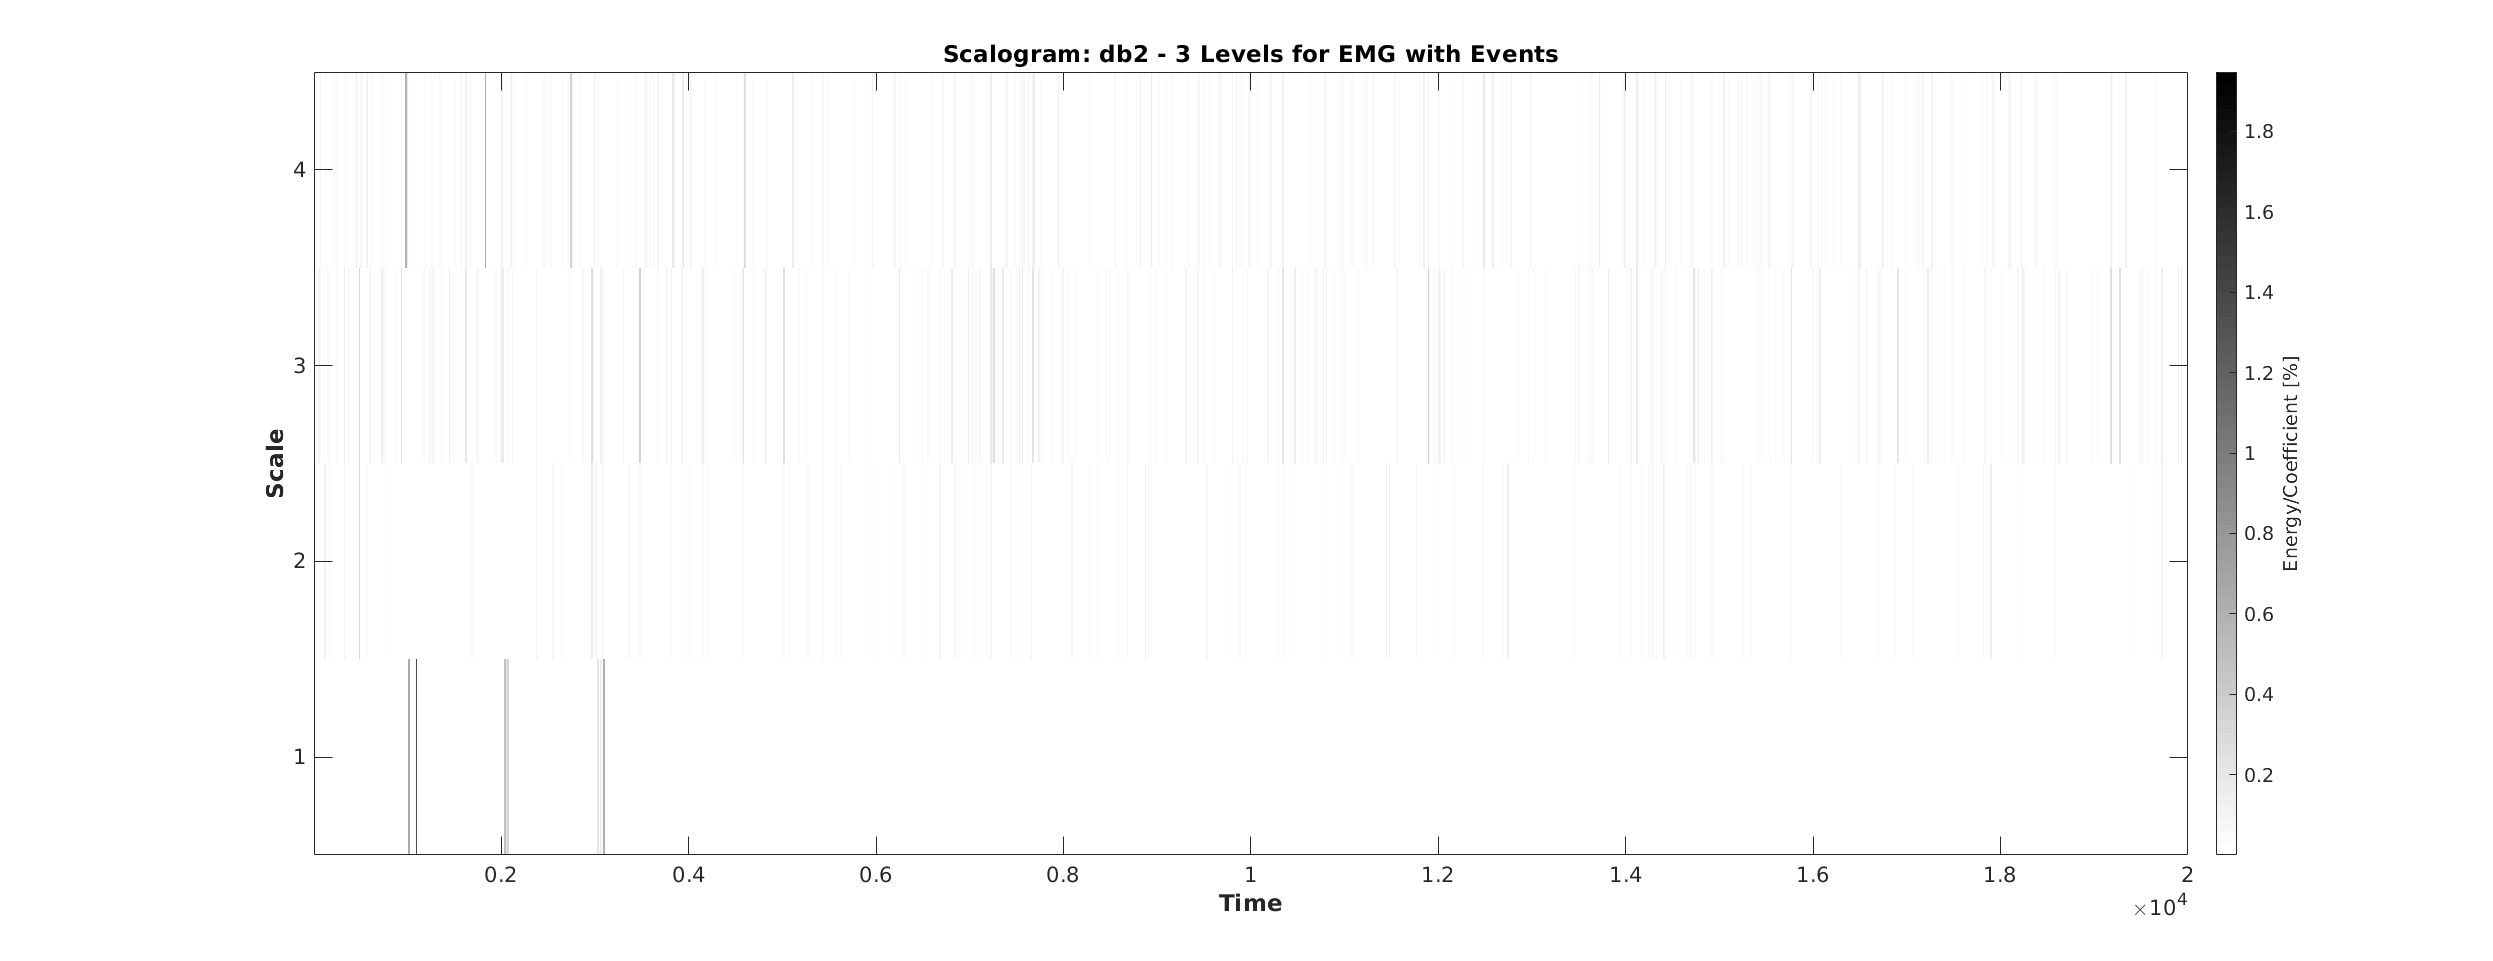
\includegraphics[scale=0.25]{../Q3_Scalo_Events.png}
		\caption{Escalograma: db2 com 3 níveis}
		\label{fig:Q3_DWT}
	\end{center}
\end{figure}

\begin{figure}[H]
	\begin{center}
		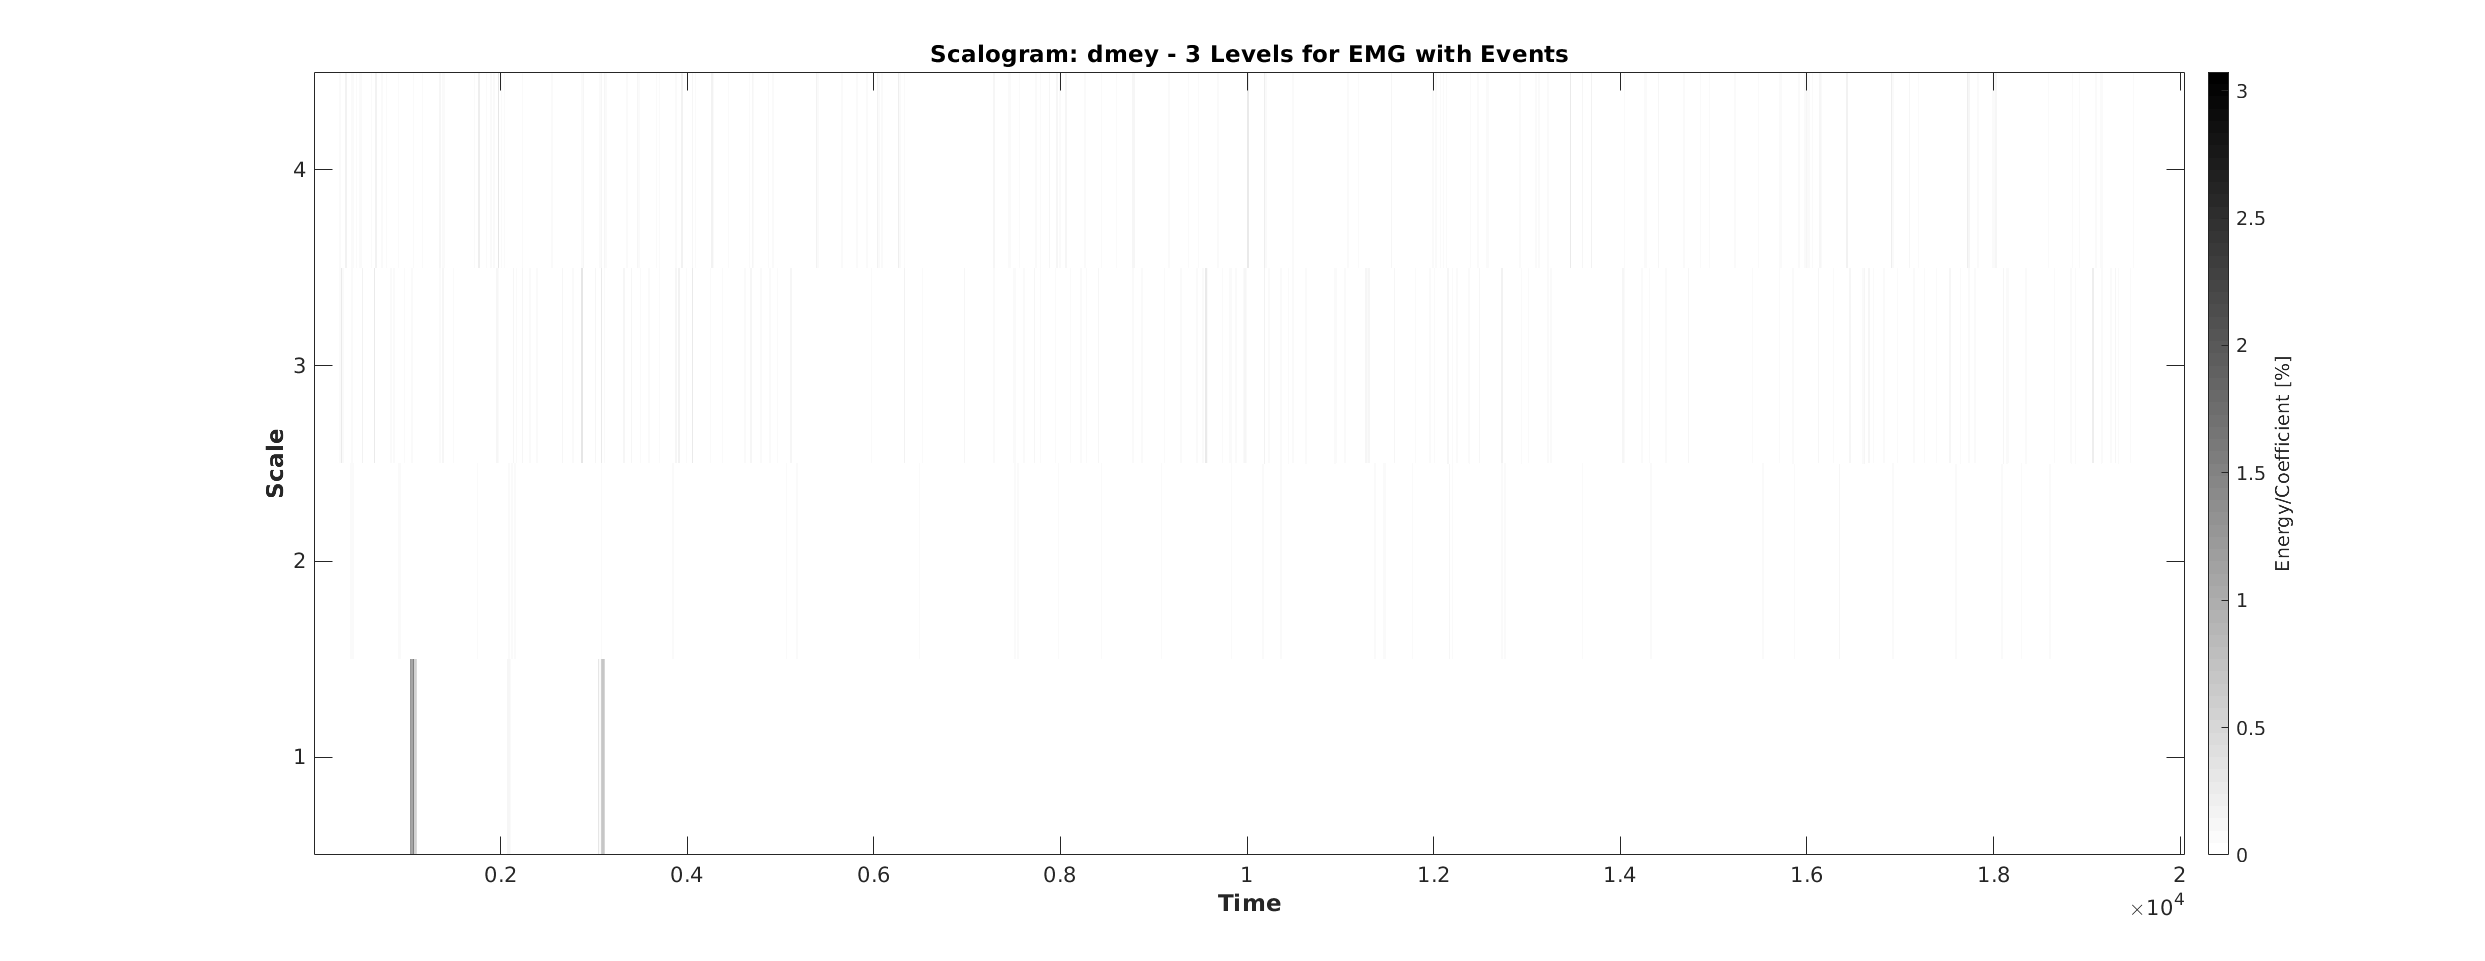
\includegraphics[scale=0.25]{../Q3_Scalo_dmey.png}
		\caption{Escalograma: dmey com 3 níveis}
		\label{fig:Q3_DWT2}
	\end{center}
\end{figure}


\subsection*{E - Comparativo: Espectrograma (STFT) vs. Escalograma (DWT)}
A figura \ref{fig:Q3_Spec} mostra o espectrograma para o sinal com a utilização da janela de Hamming com 150 ms de duração e sobreposição de 50\% entre janelas. Para o cômputo da FFT foram utilizados 512 pontos que é a próxima potência de 2 em relação ao comprimento escolhido para a janela. A figura \ref{fig:Q3_Scalo} expõe os resultados da decomposição com a família Discrete Meyer para 4 níveis. É evidente que a representação multinível detalhe muito bem os conteúdos em frequência, incluindo os eventos adicionados na menor escala. Em geral, acredito que o espectrograma seja uma ferramenta de mais fácil interpretação visual porém é preciso configurar diversos parâmetros para obter um resultado coerente. Nesse sentido, a decomposição wavelets oferece maior versatilidade.

\begin{figure}[H]
	\begin{center}
		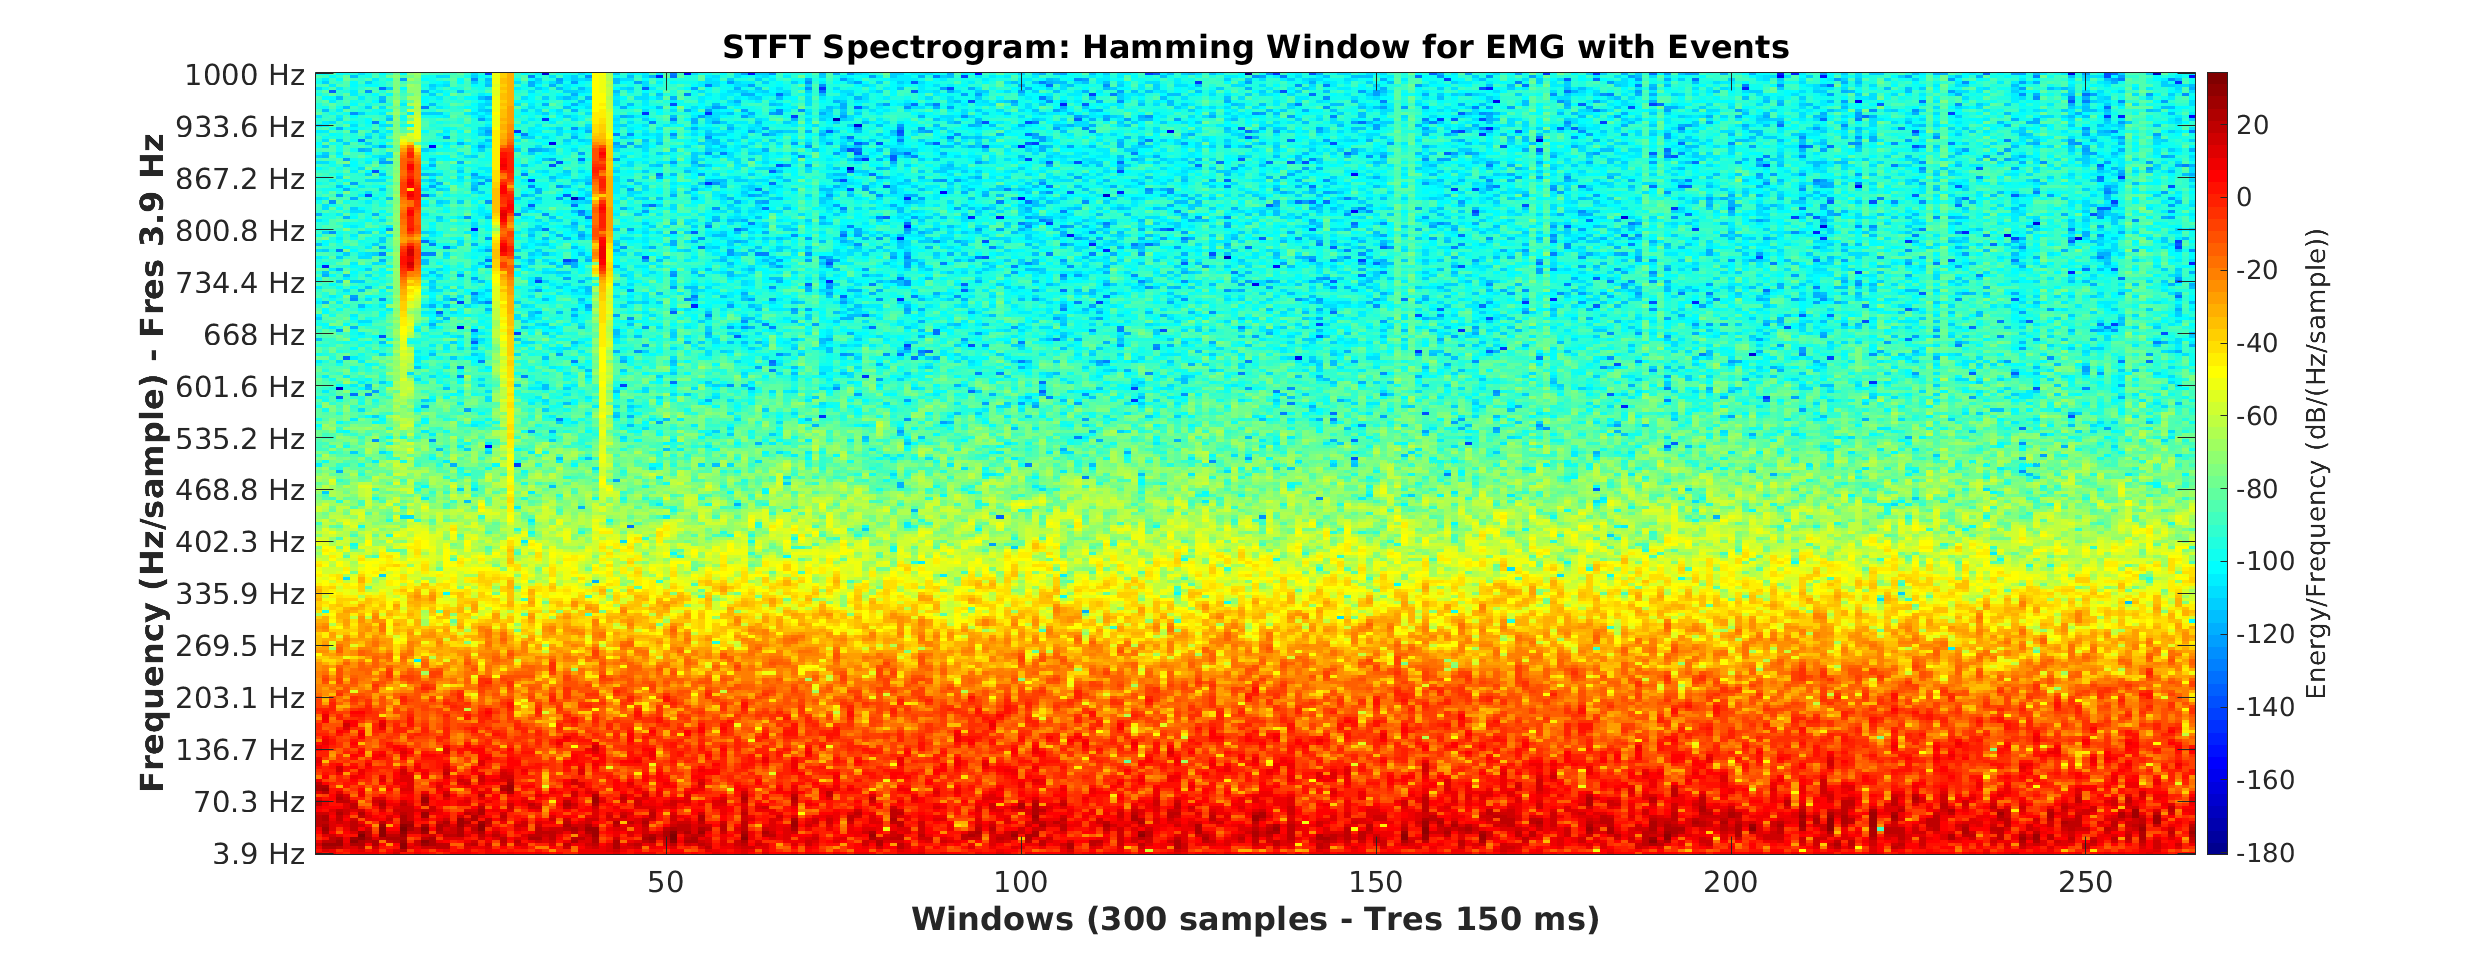
\includegraphics[scale=0.25]{../Q3_Spec.png}
		\caption{Espectrograma: Janela de Hamming com 150 ms (sobreposição de 50\%) e FFT com 512 Pontos}
		\label{fig:Q3_Spec}
	\end{center}
\end{figure}

\begin{figure}[H]
	\begin{center}
		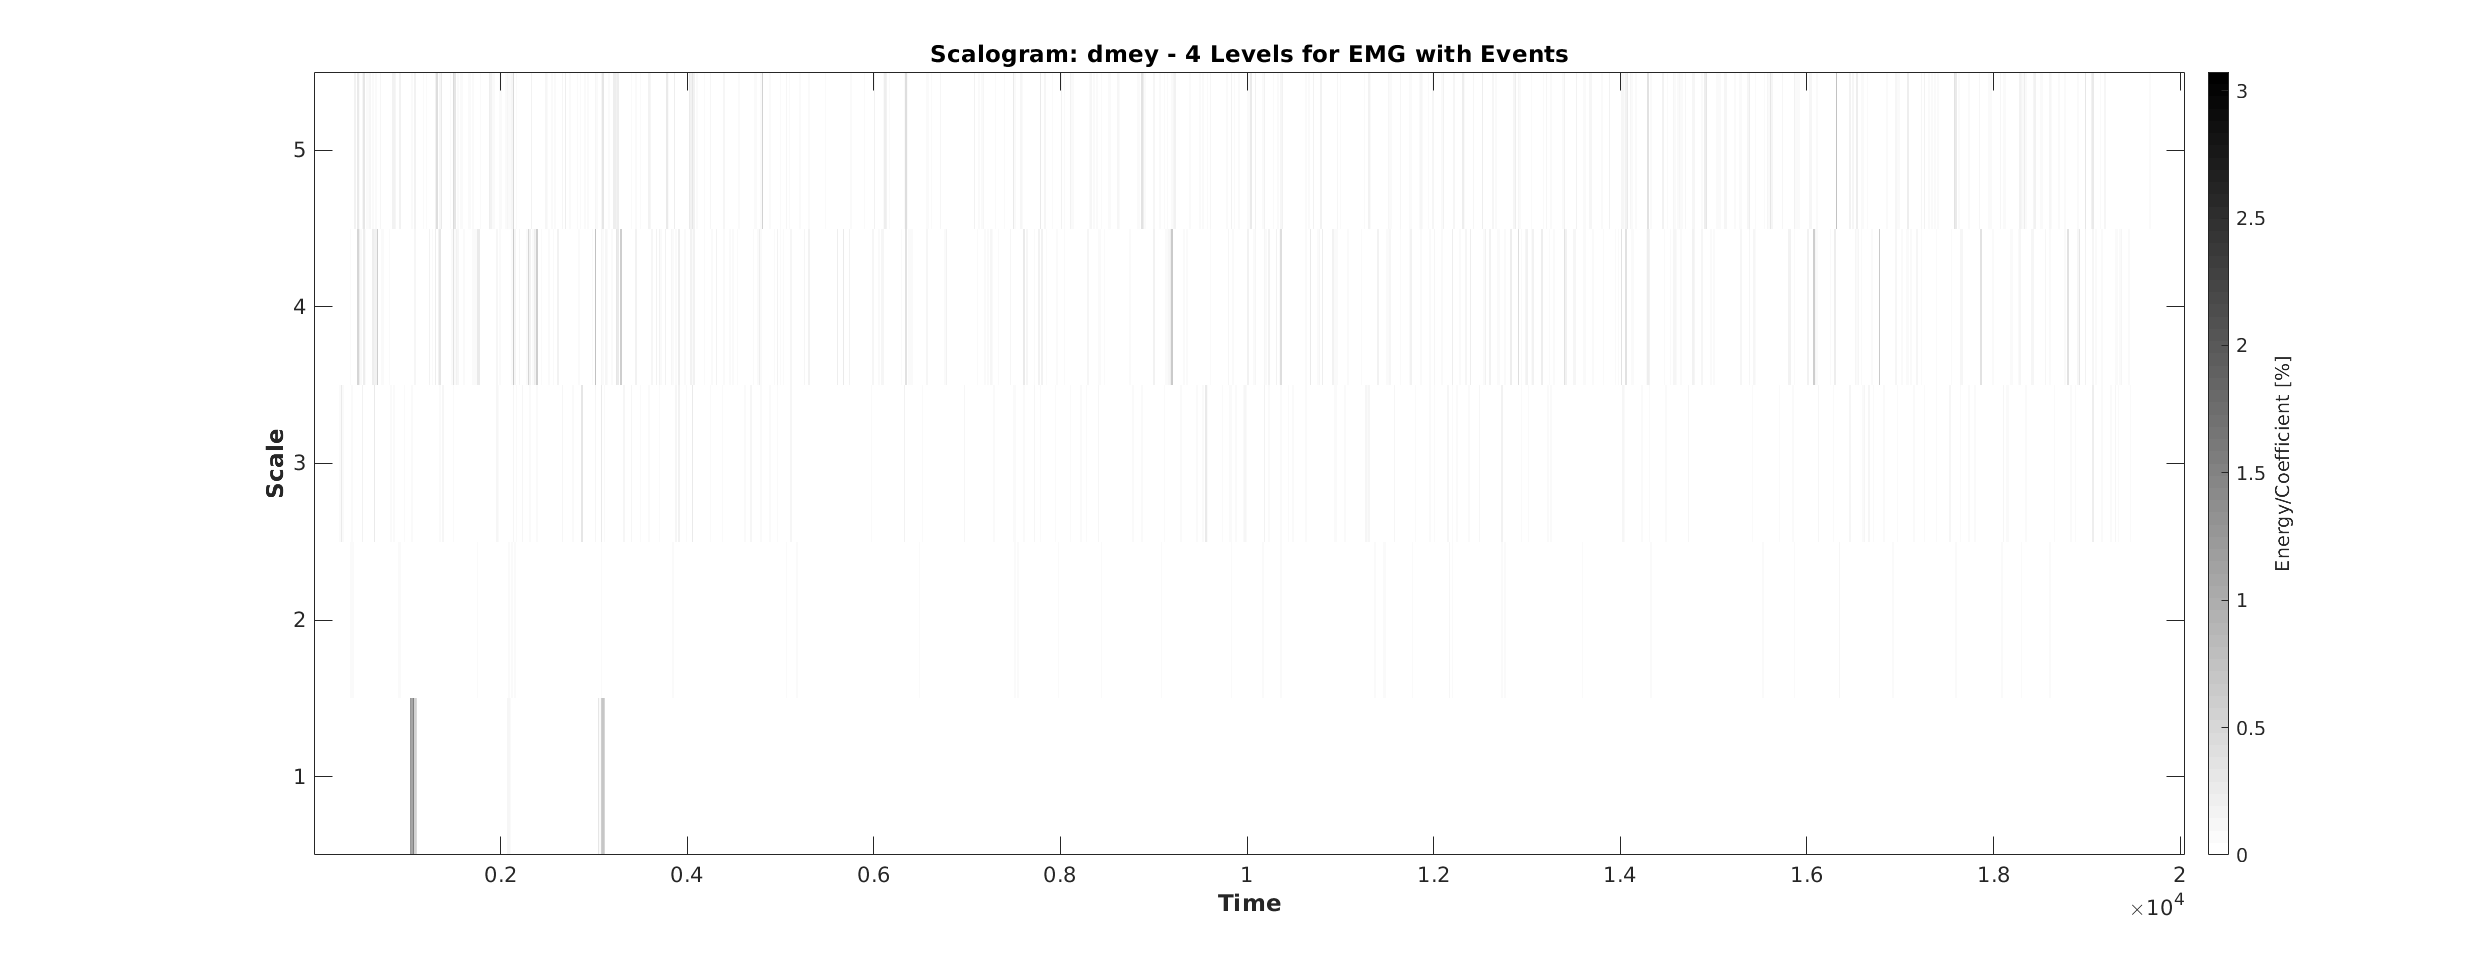
\includegraphics[scale=0.25]{../Q3_Scalo_dmey4.png}
		\caption{Escalograma: dmey com 4 níveis}
		\label{fig:Q3_Scalo}
	\end{center}
\end{figure}


% --------------------------------------------------------------------------
\section*{Questão 4 - Compressão de Sinais de ECG com DWT}
\subsection{A - Função para decomposição wavelet e quantização}
\lstinputlisting[style=Matlab-editor]{../dwtEcgQuant.m}

\subsection*{B - Síntese dos sinais de ECG quantizados}
\lstinputlisting[style=Matlab-editor]{../dwtEcgRec.m}

\subsection*{C - Visualização: SNR vs. NM \%}
% Template includegraphics
\begin{figure}[H]
	\begin{center}
		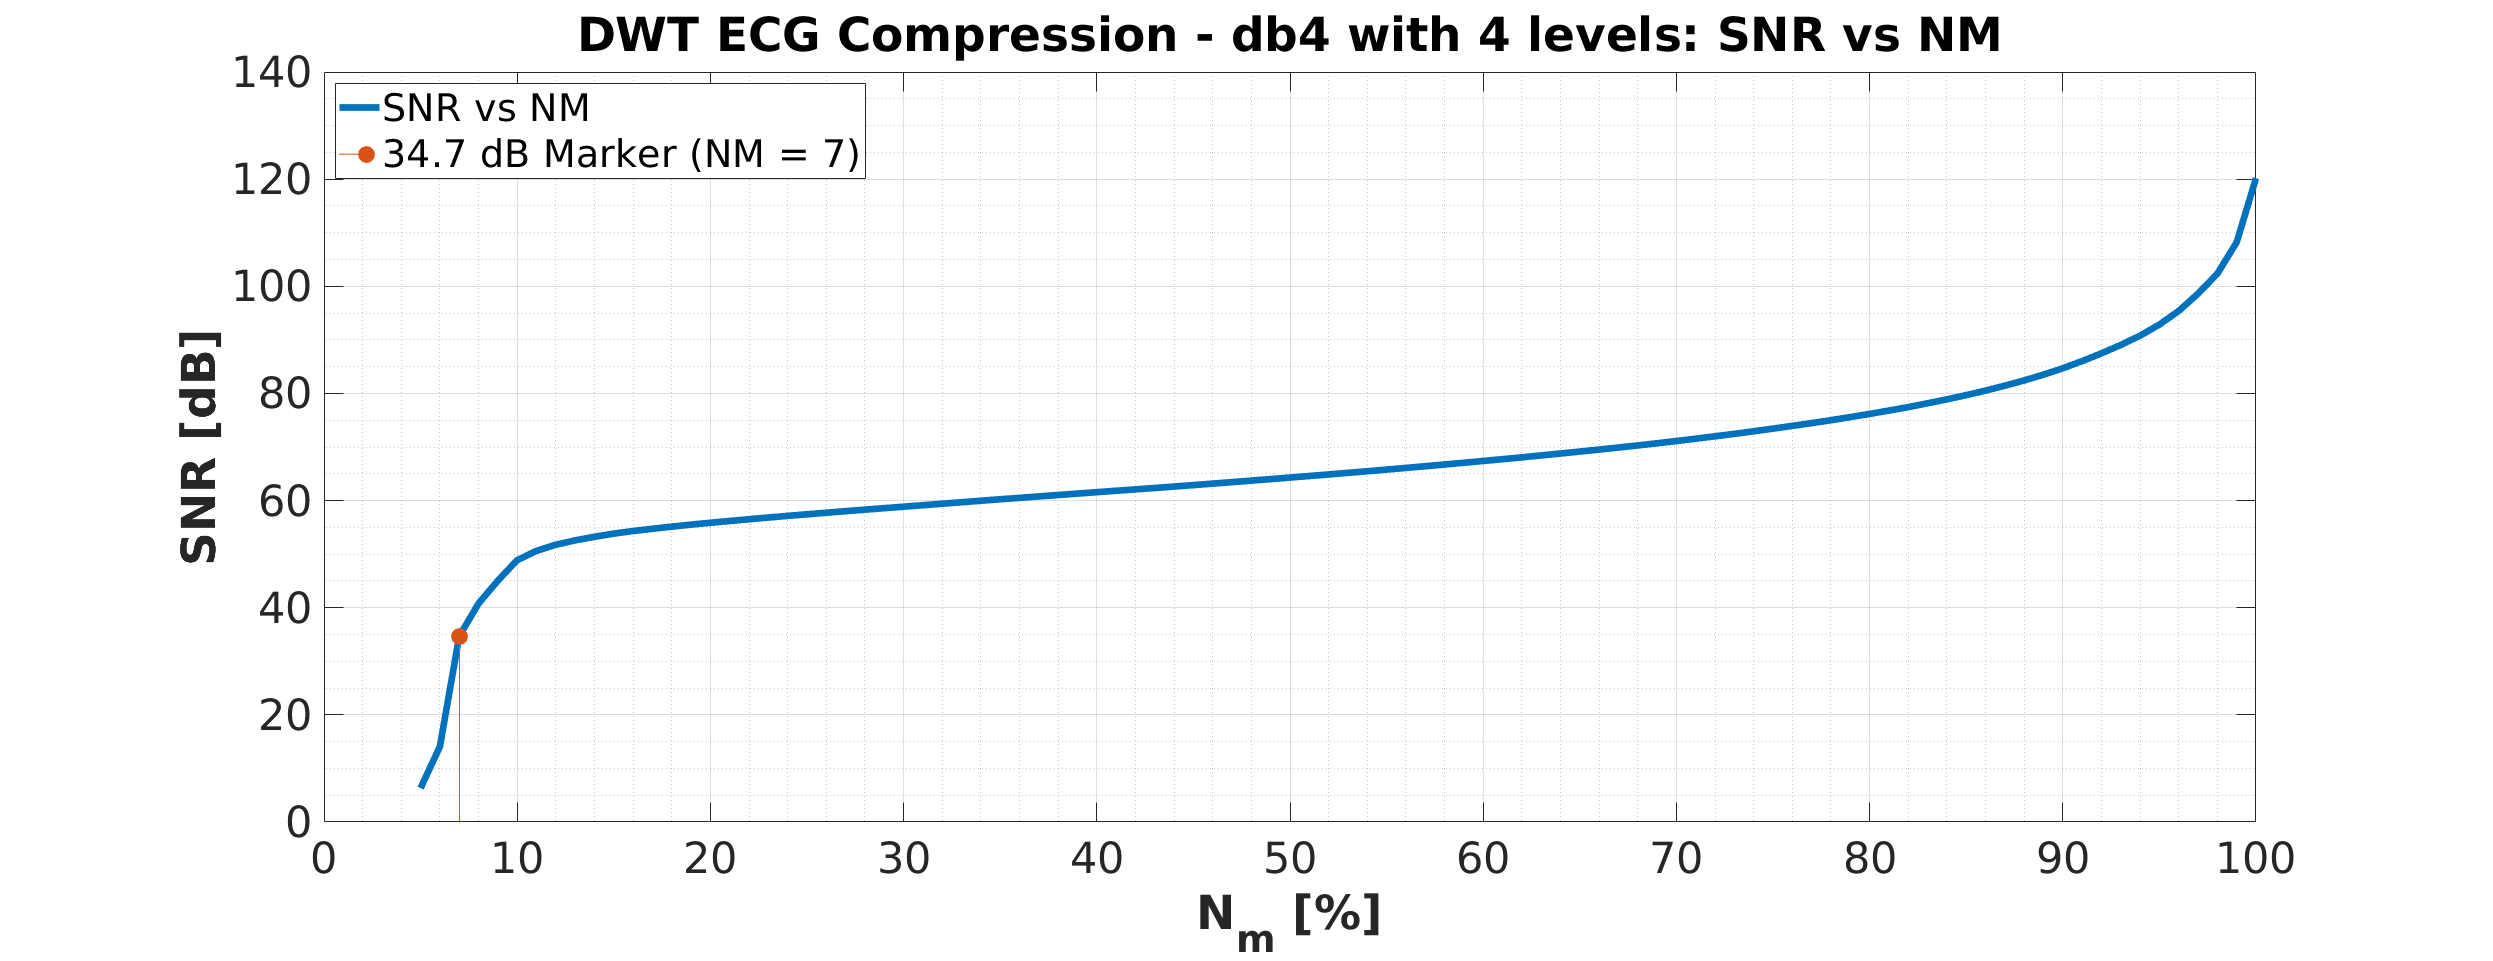
\includegraphics[scale=0.25]{../Q4_SNR-vs-NM.png}
		\caption{SNR vs. NM para Daubechies 4 (db4) com 4 níveis}
		\label{fig:Q4_SNR}
	\end{center}
\end{figure}

\begin{figure}[H]
	\begin{center}
		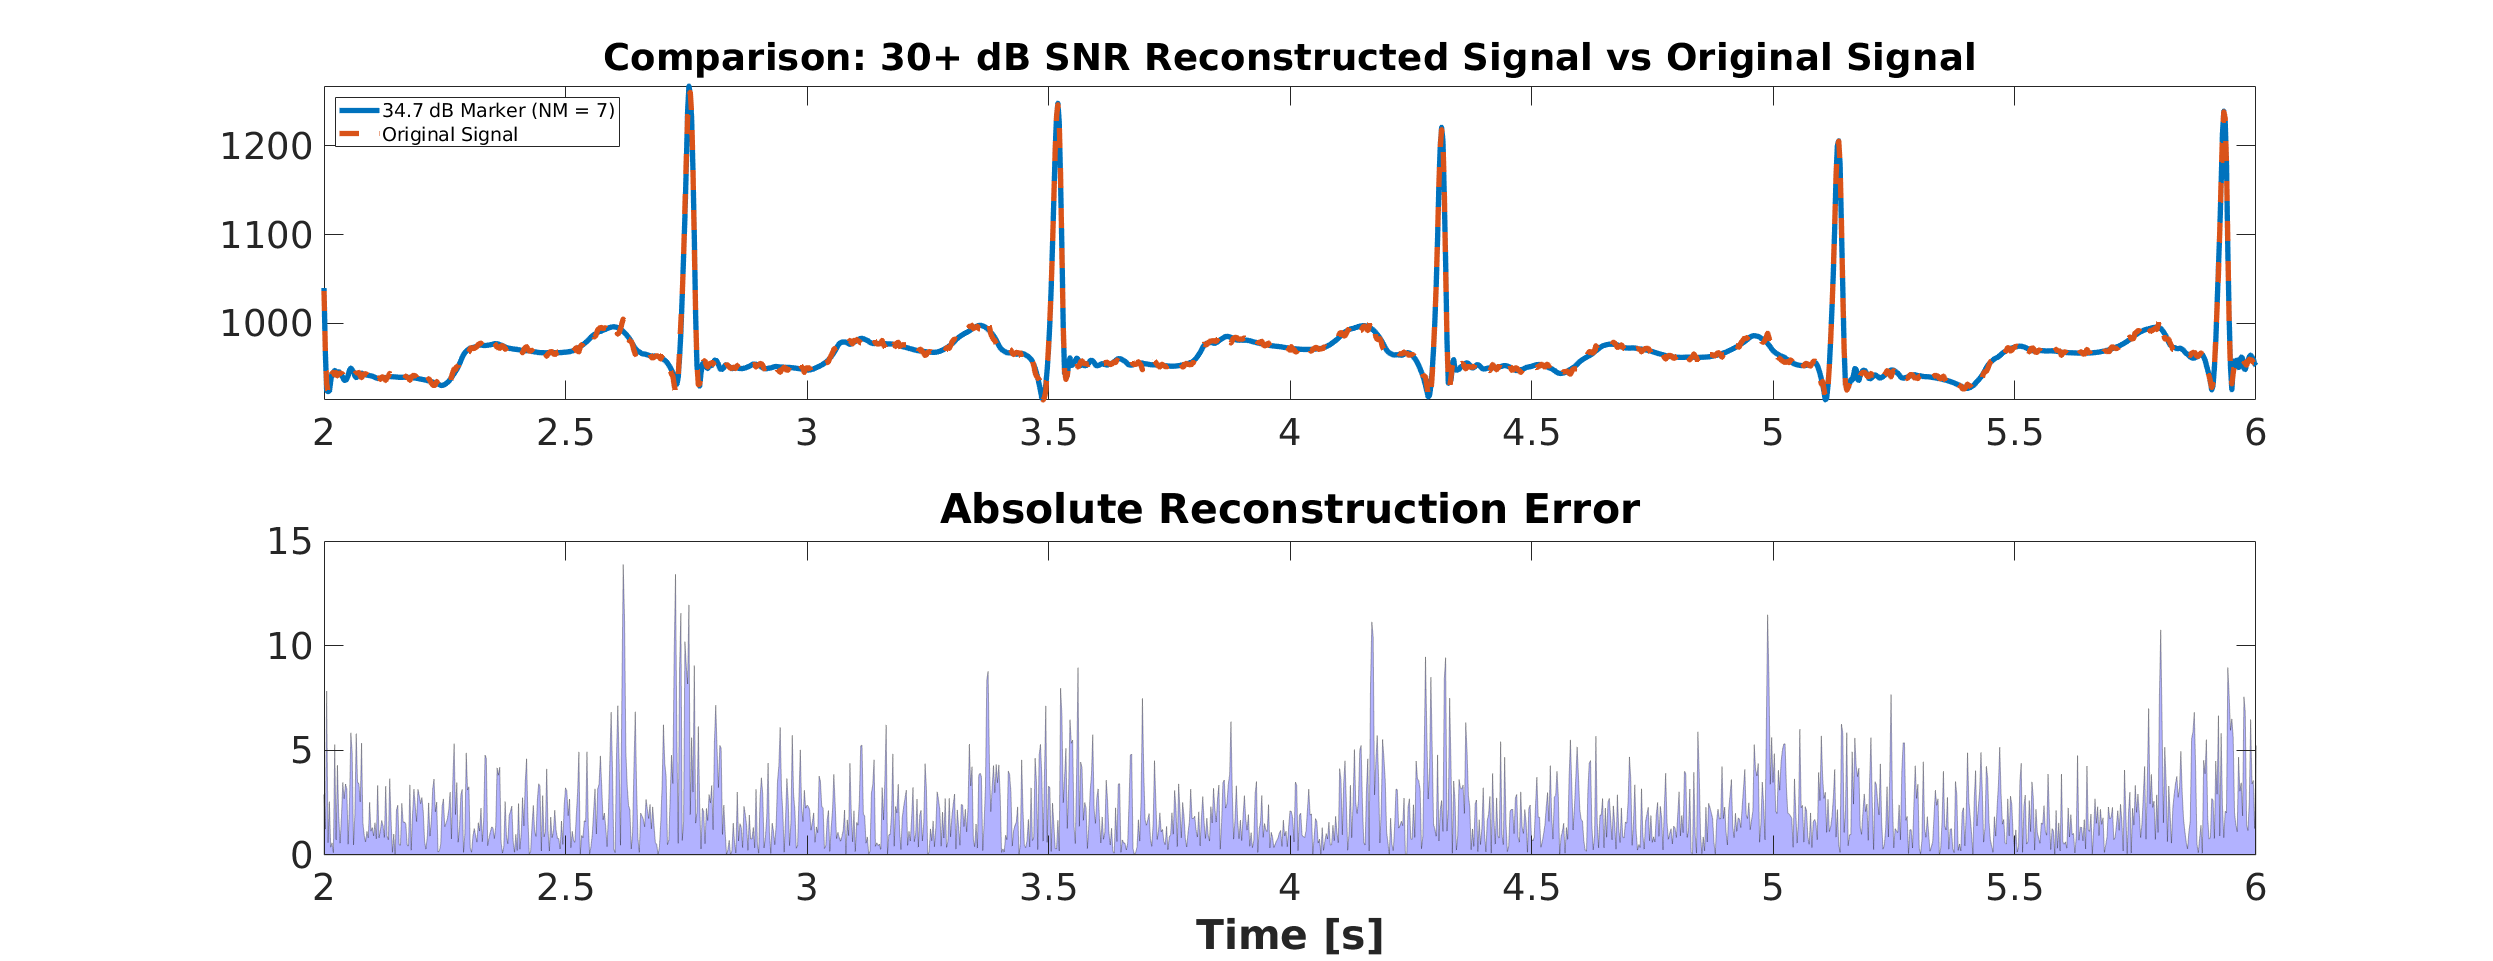
\includegraphics[scale=0.25]{../Q4_Recon-Error.png}
		\caption{Erro absoluto de reconstrução e comparação no domínio do tempo}
		\label{fig:Q4_Signal}
	\end{center}
\end{figure}

\subsection*{D - Estratégia para compressão de sinais de ECG}
\begin{multicols}{2}
Baseado na decomposição multinível utilizada sabemos que há uma elevada compactação de energia, gerando uma grande quantidade de elementos nulos em sequência para a versão quantizada da transformada. Nesse sentido, é possível utilizar a transformada quantizada aliada a um código de corrida de zeros (\textit{zero run-length}) para codificar os elementos nulos. É preciso enviar os filtros utilizados na decomposição e síntese (h0, h1, g0 e g1) além do comprimento de cada nível de decomposição de wavelets.
\end{multicols}

% --------------------------------------------------------------------------
\section*{Questão 5 - Extração de Características \& Classificação SVM}
\subsection*{A - Extração de Características - Janelas de 5 segundos para toda a banda do sinal}
A função desenvolvida está nos anexos da prova! \textbf{Para os valores presentes nas figuras ~\ref{fig:Q5_a-TF} e ~\ref{fig:Q5_a-FF} foram utilizados os sinais 1 de cada conjunto de gravações.}

\begin{figure}[H]
	\begin{center}
		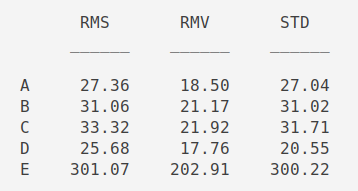
\includegraphics[scale=0.6]{Figures/Q5_a-TF.png}
		\caption{Características Temporais extraídas - Valor Eficaz, Valor Médio Retificado e Desvio Padrão (Valores Absolutos)}
		\label{fig:Q5_a-TF}
	\end{center}
\end{figure}

\begin{figure}[H]
	\begin{center}
		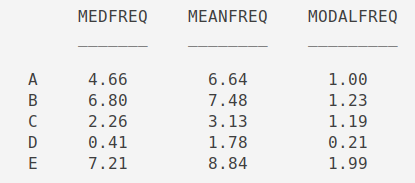
\includegraphics[scale=0.55]{Figures/Q5_a-FF.png}
		\caption{Características Espectrais extraídas - Frequência Mediana, Média e Modal (Valores em Hz)}
		\label{fig:Q5_a-FF}
	\end{center}
\end{figure}

\subsection*{B - Extração de Características por Tipo de Onda ($\delta\, \theta\, \alpha\, \beta\, \gamma$)}

\begin{figure}[H]
	\begin{center}
		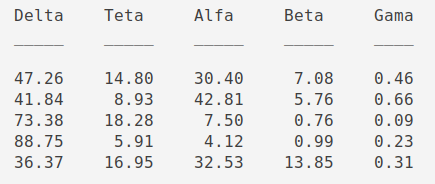
\includegraphics[scale=0.55]{Figures/Q5_b.png}
		\caption{Características Espectrais: Energia por tipo de ondas em valores percentuais em relação ao total de energia}
		\label{fig:Q5_b}
	\end{center}
\end{figure}

\subsection*{C - Extração de Características com 10 Bandas}
Para encontrar a frequência na qual há 95\% da energia do sinal basta minimizar a equação da diferença entre o valor de 95\% da energia total do sinal $x$ e sua energia na banda $0-f_m$ Hz.

\begin{lstlisting}[style=Matlab-editor]
fmfunc = @(fm) abs(0.95*bandpower(x, fs, [0 (length(x)-1)*fs/(2*length(x))]) - bandpower(x, fs, [0 fm]));
fm = fminsearch(fmfunc, 1); % Find fm starting at 1 Hz
\end{lstlisting}

\begin{figure}[H]
	\begin{center}
		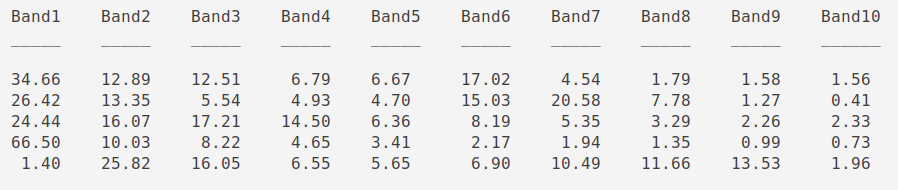
\includegraphics[scale=0.55]{Figures/Q5_c.png}
		\caption{Características Espectrais: Energia por banda em valores percentuais em relação ao total de energia}
		\label{fig:Q5_c}
	\end{center}
\end{figure}

\subsection*{D - Características Extraídas por Janela}

\begin{figure}[H]
\center
\subfigure[A1]{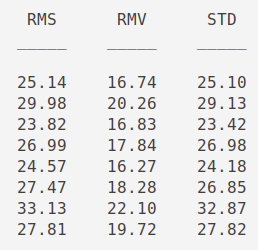
\includegraphics[width=4.5cm, height=5cm]{Figures/Q5_dA.png}\label{fig:A1}}
\qquad
\subfigure[B1]{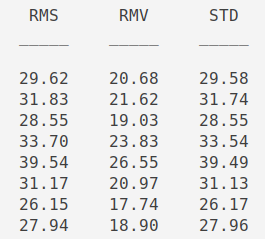
\includegraphics[width=4.5cm, height=5cm]{Figures/Q5_dB.png}\label{fig:B1}}
\qquad
\subfigure[C1]{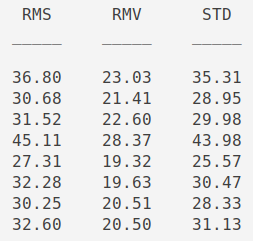
\includegraphics[width=4.5cm, height=5cm]{Figures/Q5_dC.png}\label{fig:C1}}
\qquad
\subfigure[D1]{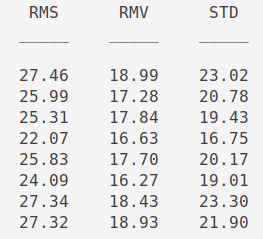
\includegraphics[width=4.5cm, height=5cm]{Figures/Q5_dD.png}\label{fig:D1}}
\qquad
\subfigure[E1]{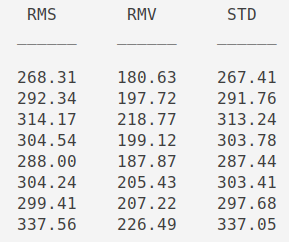
\includegraphics[width=4.5cm, height=5cm]{Figures/Q5_dE.png}\label{fig:E1}}
\caption{Características Temporais para cada Gravação em cada janela - Valor Eficaz, Valor Médio Retificado e Desvio Padrão (Valores Absolutos)}
\label{fig:Q5_dTF}
\end{figure}

\begin{figure}[H]
\center
\subfigure[A1]{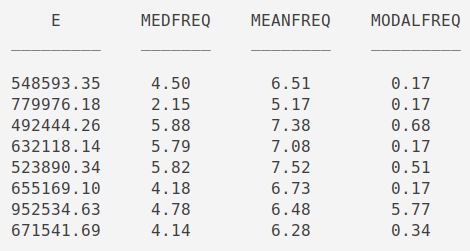
\includegraphics[width=8cm, height=5cm]{Figures/Q5_dAf.png}\label{fig:A1f}}
\qquad
\subfigure[B1]{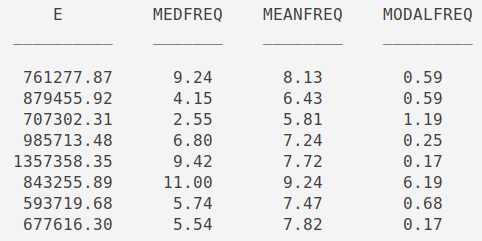
\includegraphics[width=8cm, height=5cm]{Figures/Q5_dBf.png}\label{fig:B1f}}
\qquad
\subfigure[C1]{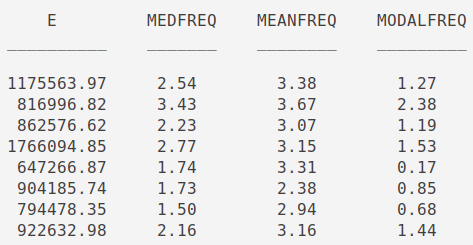
\includegraphics[width=8cm, height=5cm]{Figures/Q5_dCf.png}\label{fig:C1f}}
\qquad
\subfigure[D1]{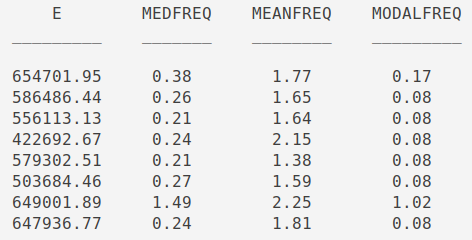
\includegraphics[width=8cm, height=5cm]{Figures/Q5_dDf.png}\label{fig:D1f}}
\qquad
\subfigure[E1]{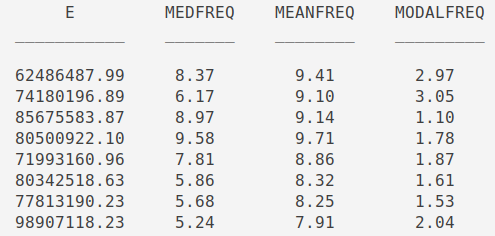
\includegraphics[width=8cm, height=5cm]{Figures/Q5_dEf.png}\label{fig:E1f}}
\caption{Características Espectrais para cada Gravação em cada janela - Energia (Valor absoluto) \& Frequência Mediana, Média e Modal (Valores em Hz)}
\label{fig:Q5_dFF}
\end{figure}

\subsection*{E - Classificação com SVM}
Para o classificador foram utilizadas as rotinas do MATLAB para 2 classes conforme o código a seguir usando reamostragem aleatória.
\lstinputlisting[style=Matlab-editor]{../svm2ClassRandperm.m}

\textbf{SVM em 1 rodada de treinamento e classificação:} As figuras ~\ref{fig:Q5_e-val1} a ~\ref{fig:Q5_e-val3} mostram as matrizes de confusão em valores percentuais de acerto para cada classe. A primeira estratégia obteve melhores acertos para a segunda classe (D) porém a terceira estratégia obteve resultados mais uniformes para ambas as classes com mais de 95\% de acerto em cada classe. \textbf{Para o conjunto de treinamento foram usados 80\% dos dados disponíveis.}

\begin{figure}[H]
	\begin{center}
		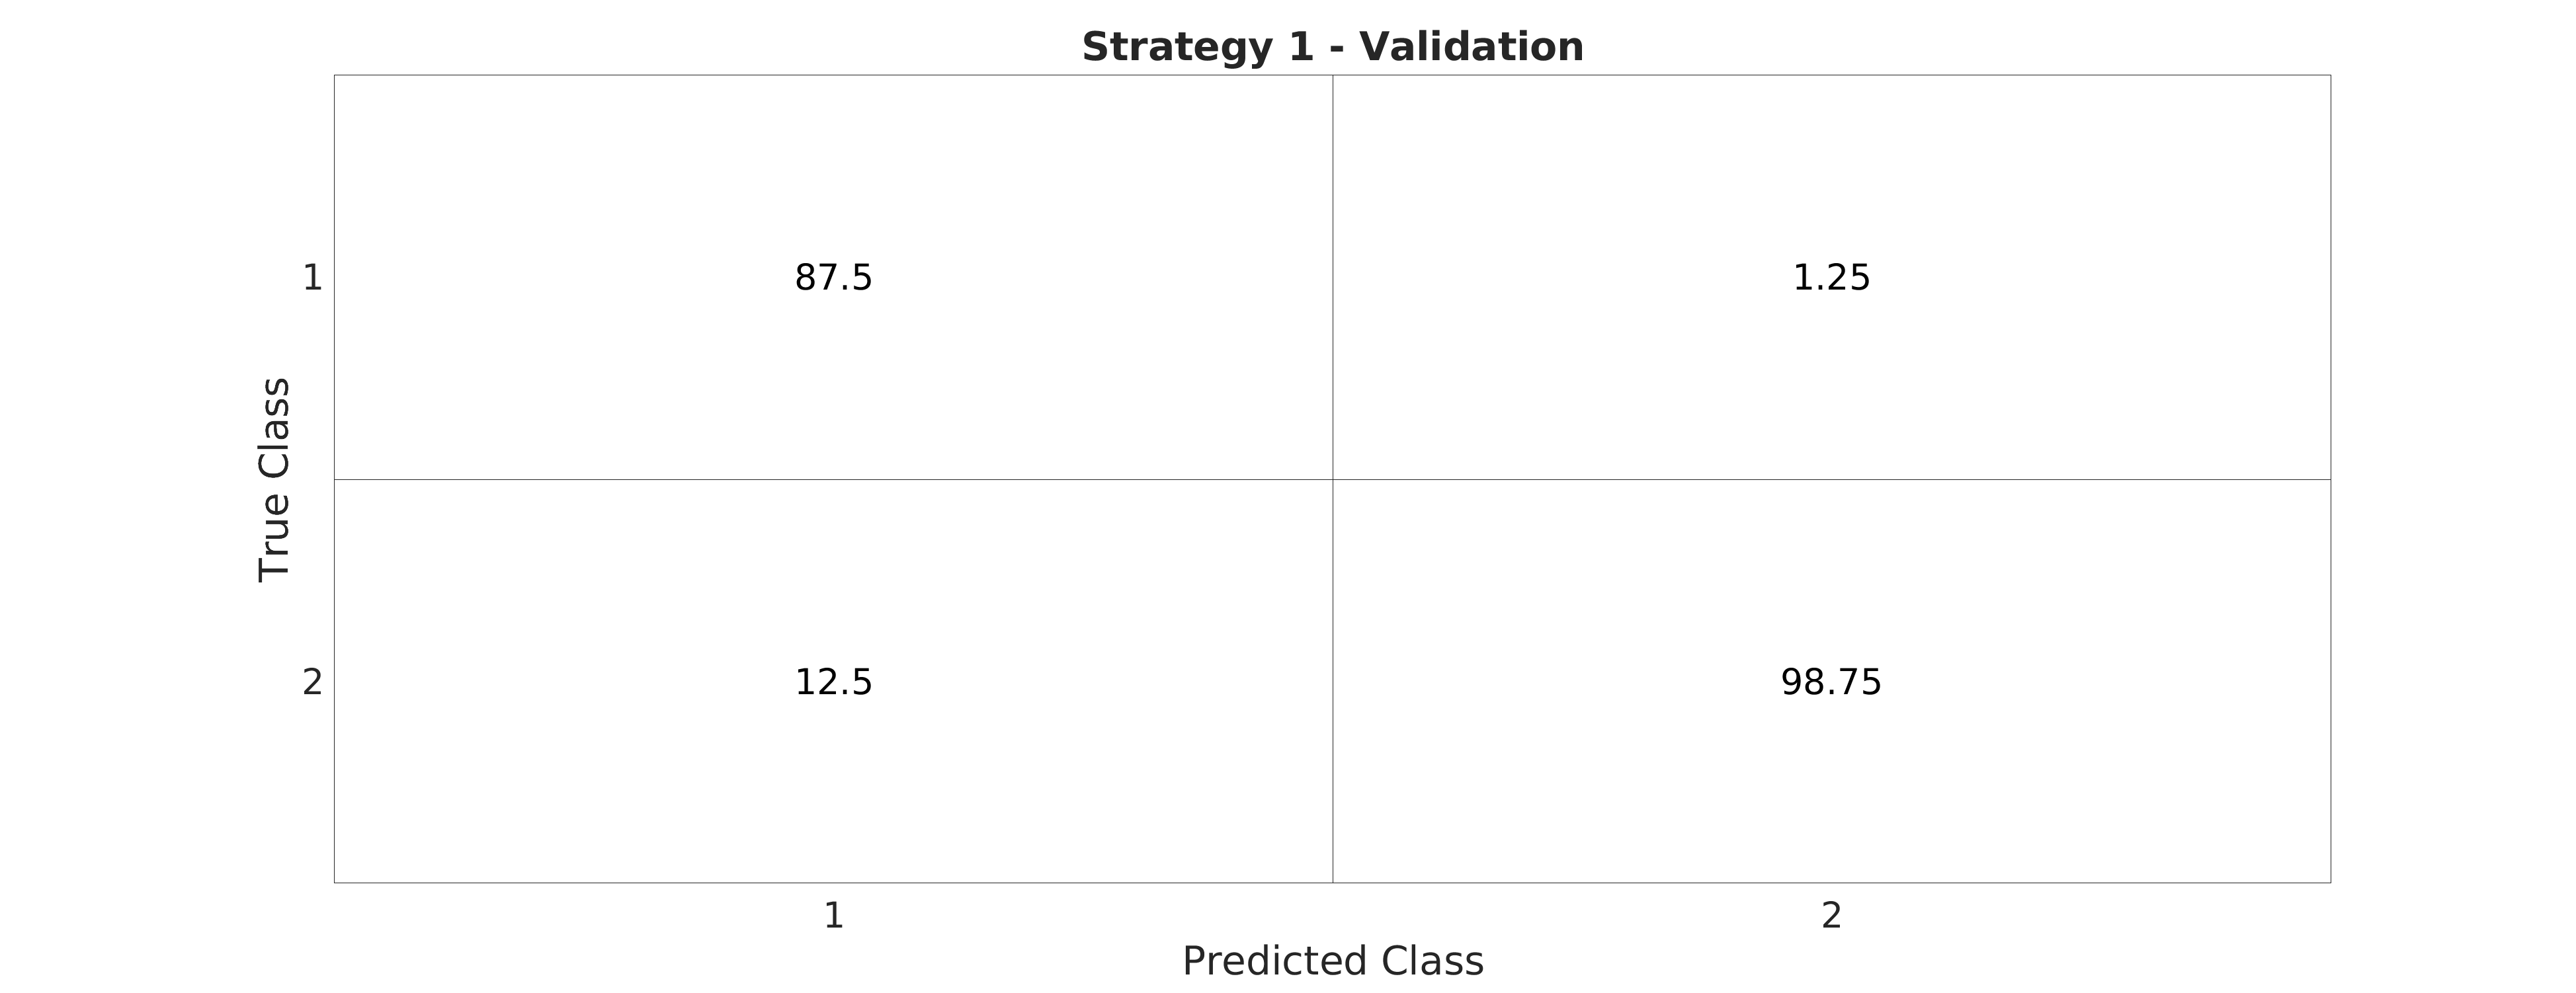
\includegraphics[scale=0.2]{../Q5_e-val1.png}
		\caption{\textit{Confusion Matrix Chart:} Estratégia 1 - Energias de bandas ($\delta\, \theta\, \alpha\, \beta\, \gamma$)}
		\label{fig:Q5_e-val1}
	\end{center}
\end{figure}

\begin{figure}[H]
	\begin{center}
		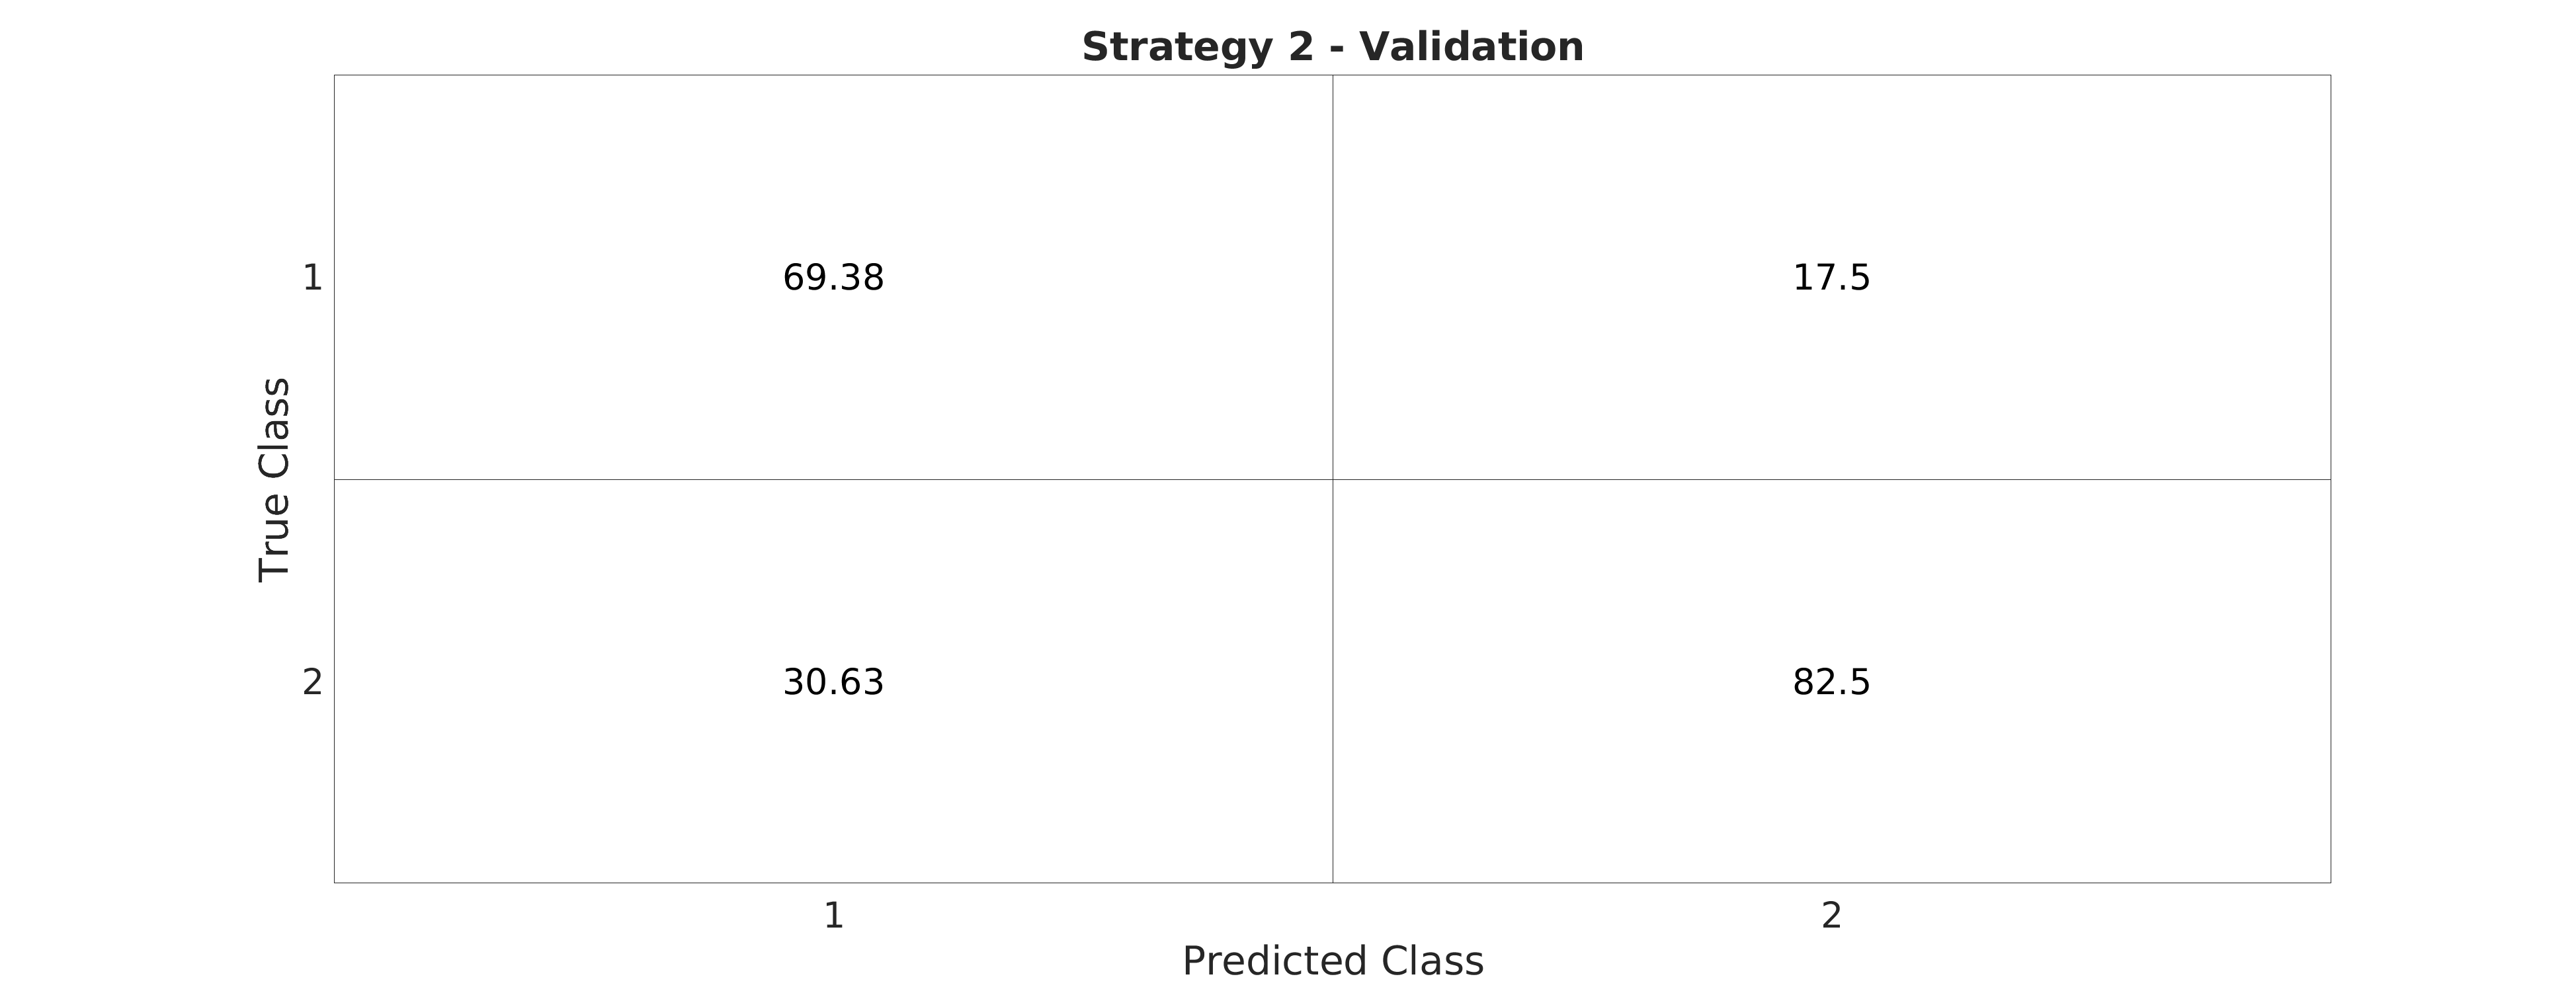
\includegraphics[scale=0.2]{../Q5_e-val2.png}
		\caption{\textit{Confusion Matrix Chart:} Estratégia 2 - Energia em 10 bandas consecutivas}
		\label{fig:Q5_e-val2}
	\end{center}
\end{figure}

\begin{figure}[H]
	\begin{center}
		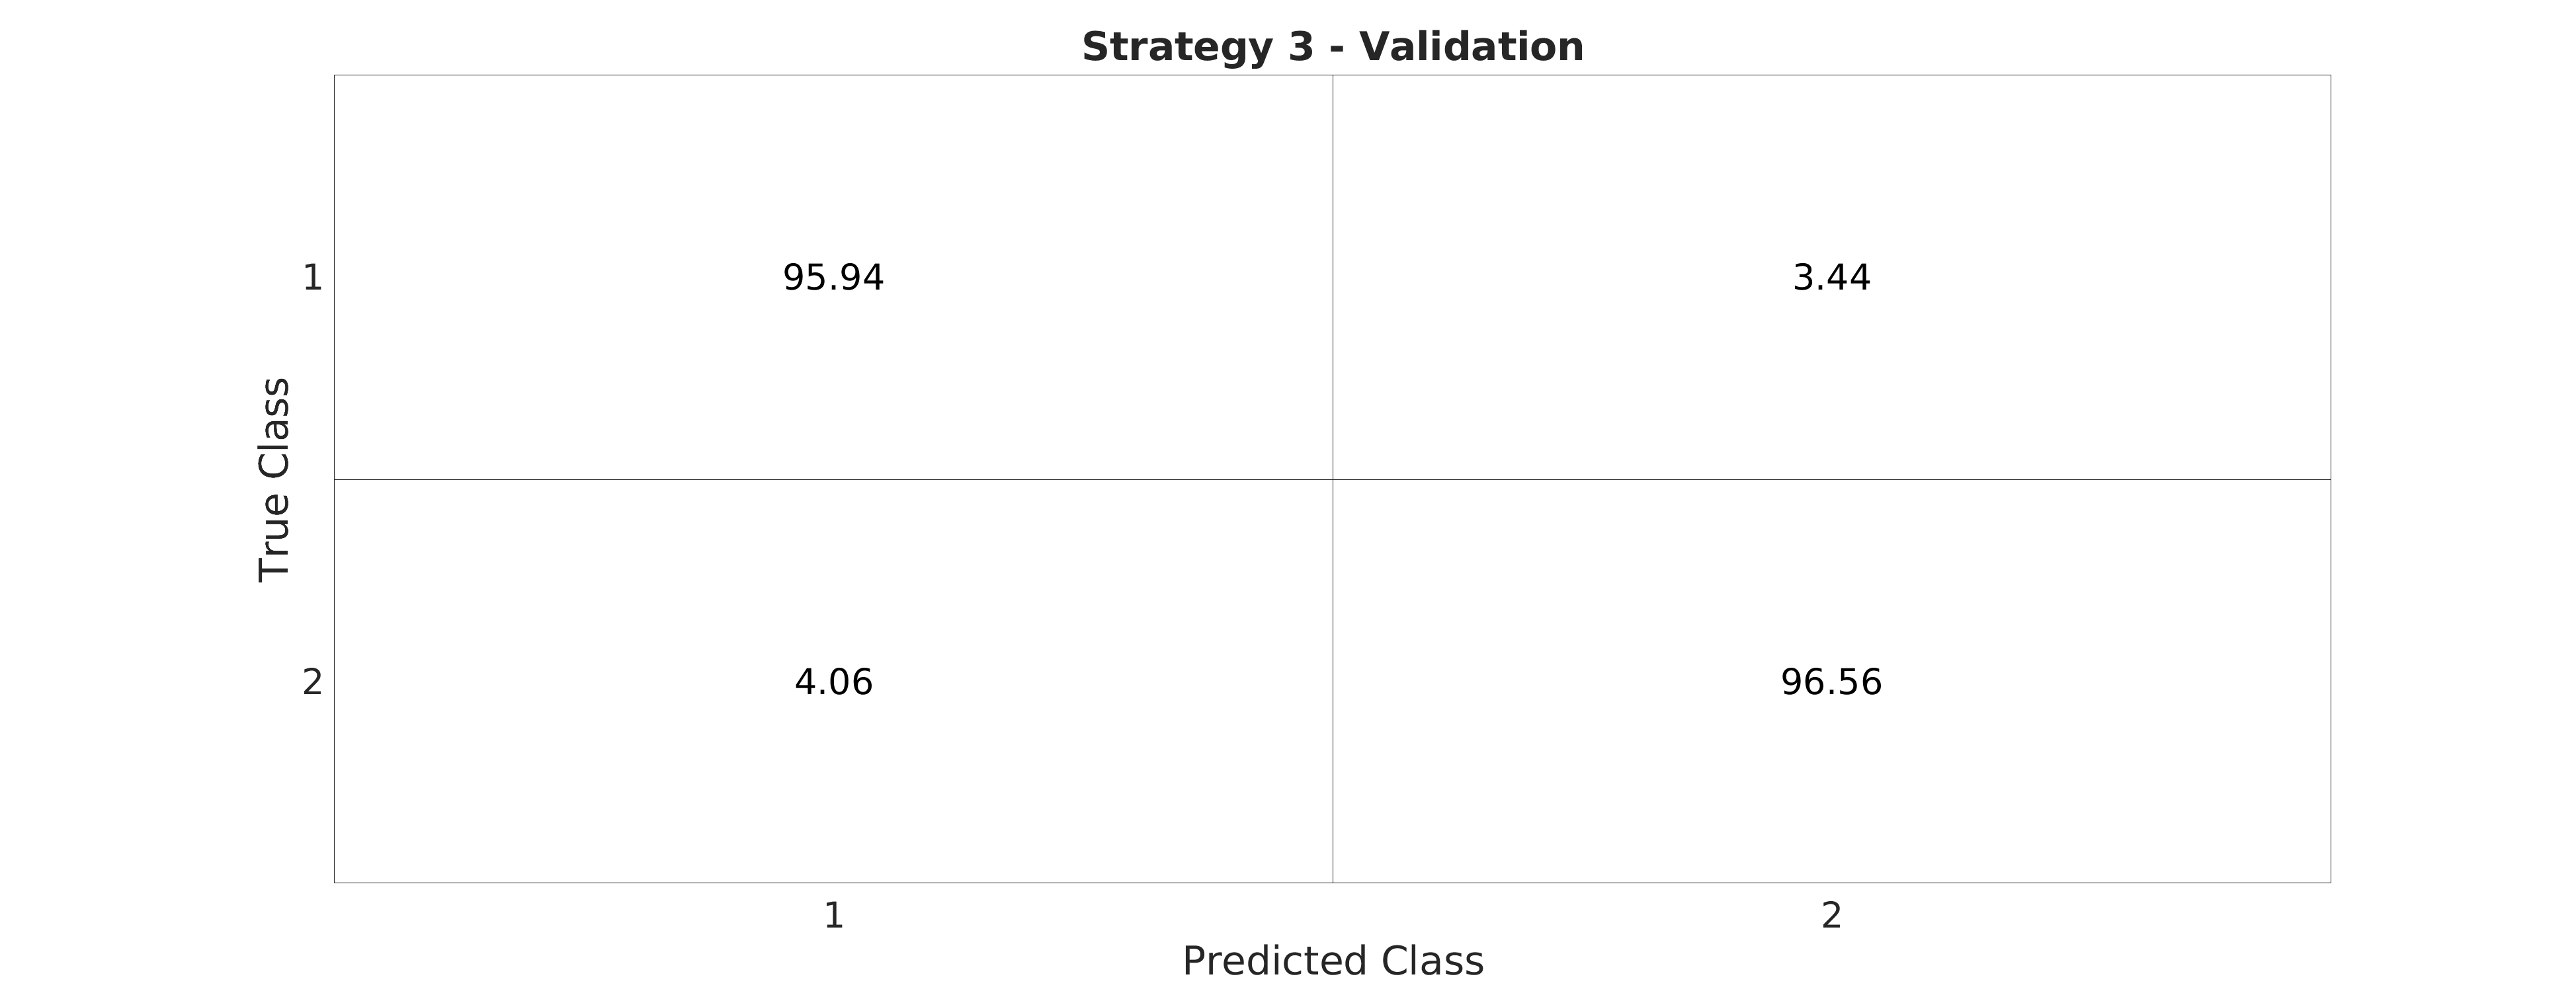
\includegraphics[scale=0.2]{../Q5_e-val3.png}
		\caption{\textit{Confusion Matrix Chart:} Estratégia 3 - Valor Eficaz \& Frequência Média, Mediana e Modal}
		\label{fig:Q5_e-val3}
	\end{center}
\end{figure}

\subsection*{F - SVM com Reamostragem Aleatória em 500 sessões}
As figuras ~\ref{fig:Q5_ROC} e ~\ref{fig:Q5_M} dispõe os resultados obtidos para o classificador em 500 sessões de treinamento e validação com reamostragem aleatória. De maneira geral a estratégia 3 que utiliza a energia em bandas ($\delta\, \theta\, \alpha\, \beta\, \gamma$) resulta em melhores resultados para as métricas avaliadas. A estratégia 2 com energias em 10 bandas consecutivas, embora similar a estratégia 2, resulta em pouca convergência com índices bem menos expressivos. A estratégia 1 aproxima-se bastante dos melhores resultados por empregar frequências médias, modais e medianas além dos valores eficazes para as janelas consideradas.


\begin{figure}[H]
	\begin{center}
		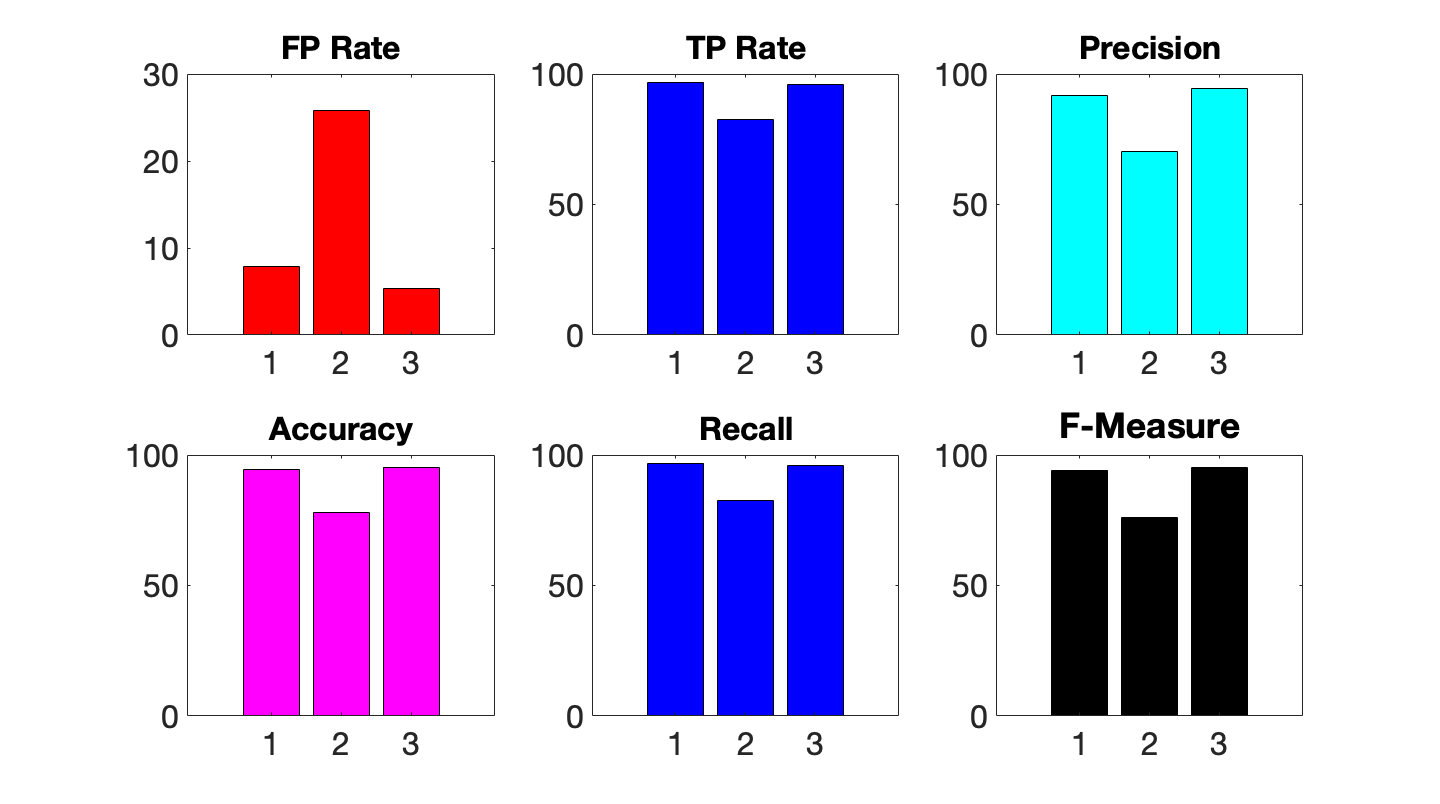
\includegraphics[scale=0.3]{../Q5_f.png}
		\caption{Métricas para o Classificador Obtido}
		\label{fig:Q5_ROC}
	\end{center}
\end{figure}

\begin{figure}[H]
\center
\subfigure[E1]{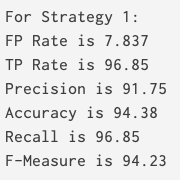
\includegraphics[width=4.5cm, height=5cm]{Figures/Q5_f1.png}}
\qquad
\subfigure[E2]{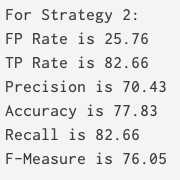
\includegraphics[width=4.5cm, height=5cm]{Figures/Q5_f2.png}}
\qquad
\subfigure[E3]{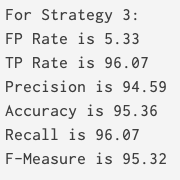
\includegraphics[width=4.5cm, height=5cm]{Figures/Q5_f3.png}}
\caption{Métricas para cada uma das estratégias utilizadas}
\label{fig:Q5_M}
\end{figure}

\section*{Considerações Finais}
O desenvolvimento da prova foi bastante proveitoso para consolidar conceitos fundamentais e aplicar diferentes técnicas de processamento de sinais biológicos para filtragem, codificação \& compressão em sinais de ECG, extração \& escolha de características e classificação com SVM. Estimo que o tempo total de desenvolvimento da prova tenha tomado em torno de 13 horas para conclusão das questões incluindo o tempo necessário para redigir a parte textual da prova. Finalmente, espero que tenha gostado dos resultados obtidos.

\textbf{Davi Mendes}

\newpage
\section*{Anexos}

\subsection*{Q2 - Rotina computacional para visualização dos dados e filtragem FIR \& DFT}
\lstinputlisting[style=Matlab-editor]{../Q2.m}

\subsection*{Q3 - Espectrograma (STFT)}
\lstinputlisting[style=Matlab-editor]{../../utils_P1/stftSpectrogram.m}

\subsection*{Q3 - Escalograma (DWT)}
\lstinputlisting[style=Matlab-editor]{../../utils_P1/dwtScalogram.m}

\subsection*{Q3 - Rotina computacional para visualização dos gráficos da Questão 3}
\lstinputlisting[style=Matlab-editor]{../Q3.m}

\subsection*{Q4 - Código para cômputo das métricas e gráficos}
\lstinputlisting[style=Matlab-editor]{../Q4.m}

\subsection*{Q5 - Extrator de características (Temporais \& Espectrais)}
\lstinputlisting[style=Matlab-editor]{../../utils_P1/featureExtractor.m}

\subsection*{Q5 - Rotina para Características de acordo com Estratégia}
\lstinputlisting[style=Matlab-editor]{../Q5_allFeatures.m}

\subsection*{Q5 - Rotina para classificação em 500 sessões de treinamento}
\lstinputlisting[style=Matlab-editor]{../Q5_svmClassify.m}

% -------------------------------------------------------------------------
% \begin{thebibliography}{1}

% \end{thebibliography}
\end{document}
